%%%%%%%%%%%%%%%%%%%%%%%%%%%%%%%%%%%%%%%%%%%%%%%%%%%%%%%%%%%%%%%%%%%%%%%%%%%%%%%%
% Template for USENIX papers.
%
% History:
%
% - TEMPLATE for Usenix papers, specifically to meet requirements of
%   USENIX '05. originally a template for producing IEEE-format
%   articles using LaTeX. written by Matthew Ward, CS Department,
%   Worcester Polytechnic Institute. adapted by David Beazley for his
%   excellent SWIG paper in Proceedings, Tcl 96. turned into a
%   smartass generic template by De Clarke, with thanks to both the
%   above pioneers. Use at your own risk. Complaints to /dev/null.
%   Make it two column with no page numbering, default is 10 point.
%
% - Munged by Fred Douglis <douglis@research.att.com> 10/97 to
%   separate the .sty file from the LaTeX source template, so that
%   people can more easily include the .sty file into an existing
%   document. Also changed to more closely follow the style guidelines
%   as represented by the Word sample file.
%
% - Note that since 2010, USENIX does not require endnotes. If you
%   want foot of page notes, don't include the endnotes package in the
%   usepackage command, below.
% - This version uses the latex2e styles, not the very ancient 2.09
%   stuff.
%
% - Updated July 2018: Text block size changed from 6.5" to 7"
%
% - Updated Dec 2018 for ATC'19:
%
%   * Revised text to pass HotCRP's auto-formatting check, with
%     hotcrp.settings.submission_form.body_font_size=10pt, and
%     hotcrp.settings.submission_form.line_height=12pt
%
%   * Switched from \endnote-s to \footnote-s to match Usenix's policy.
%
%   * \section* => \begin{abstract} ... \end{abstract}
%
%   * Make template self-contained in terms of bibtex entires, to allow
%     this file to be compiled. (And changing refs style to 'plain'.)
%
%   * Make template self-contained in terms of figures, to
%     allow this file to be compiled.
%
%   * Added packages for hyperref, embedding fonts, and improving
%     appearance.
%
%   * Removed outdated text.
%
%%%%%%%%%%%%%%%%%%%%%%%%%%%%%%%%%%%%%%%%%%%%%%%%%%%%%%%%%%%%%%%%%%%%%%%%%%%%%%%%

\documentclass[letterpaper,twocolumn,10pt]{article}
\usepackage{usenix-2020-09}

% to be able to draw some self-contained figs
\usepackage{tikz}
\usepackage{amsmath}
\usepackage{subfig}

% use for decent code formatting
\usepackage{inconsolata}
\usepackage[outputdir=build]{minted}


% notes for different people
\newcommand{\tg}[1]{\ifisdraft{\color{blue}[#1 -- Todd]}\fi}
\newcommand{\spack}{\texttt{Spack}}
\newcommand{\clingo}{\texttt{clingo}}
\definecolor{bg}{rgb}{0.95,0.95,0.95}
%-------------------------------------------------------------------------------
\begin{document}
%-------------------------------------------------------------------------------

%don't want date printed
\date{}

% make title bold and 14 pt font (Latex default is non-bold, 16 pt)
\title{\Large \bf Formatting Submissions for a USENIX Conference:\\
  An (Incomplete) Example}

%for single author (just remove % characters)
\author{
{\rm Your N.\ Here}\\
Your Institution
\and
{\rm Second Name}\\
Second Institution
% copy the following lines to add more authors
% \and
% {\rm Name}\\
%Name Institution
} % end author

\maketitle

\begin{abstract}
Your abstract text goes here. Just a few facts. Whet our appetites.
Not more than 200 words, if possible, and preferably closer to 150.
\end{abstract}

%-------------------------------------------------------------------------------
\section{Introduction}
%-------------------------------------------------------------------------------
\label{sec:intro}


%\begin{figure}
%  \centering
%  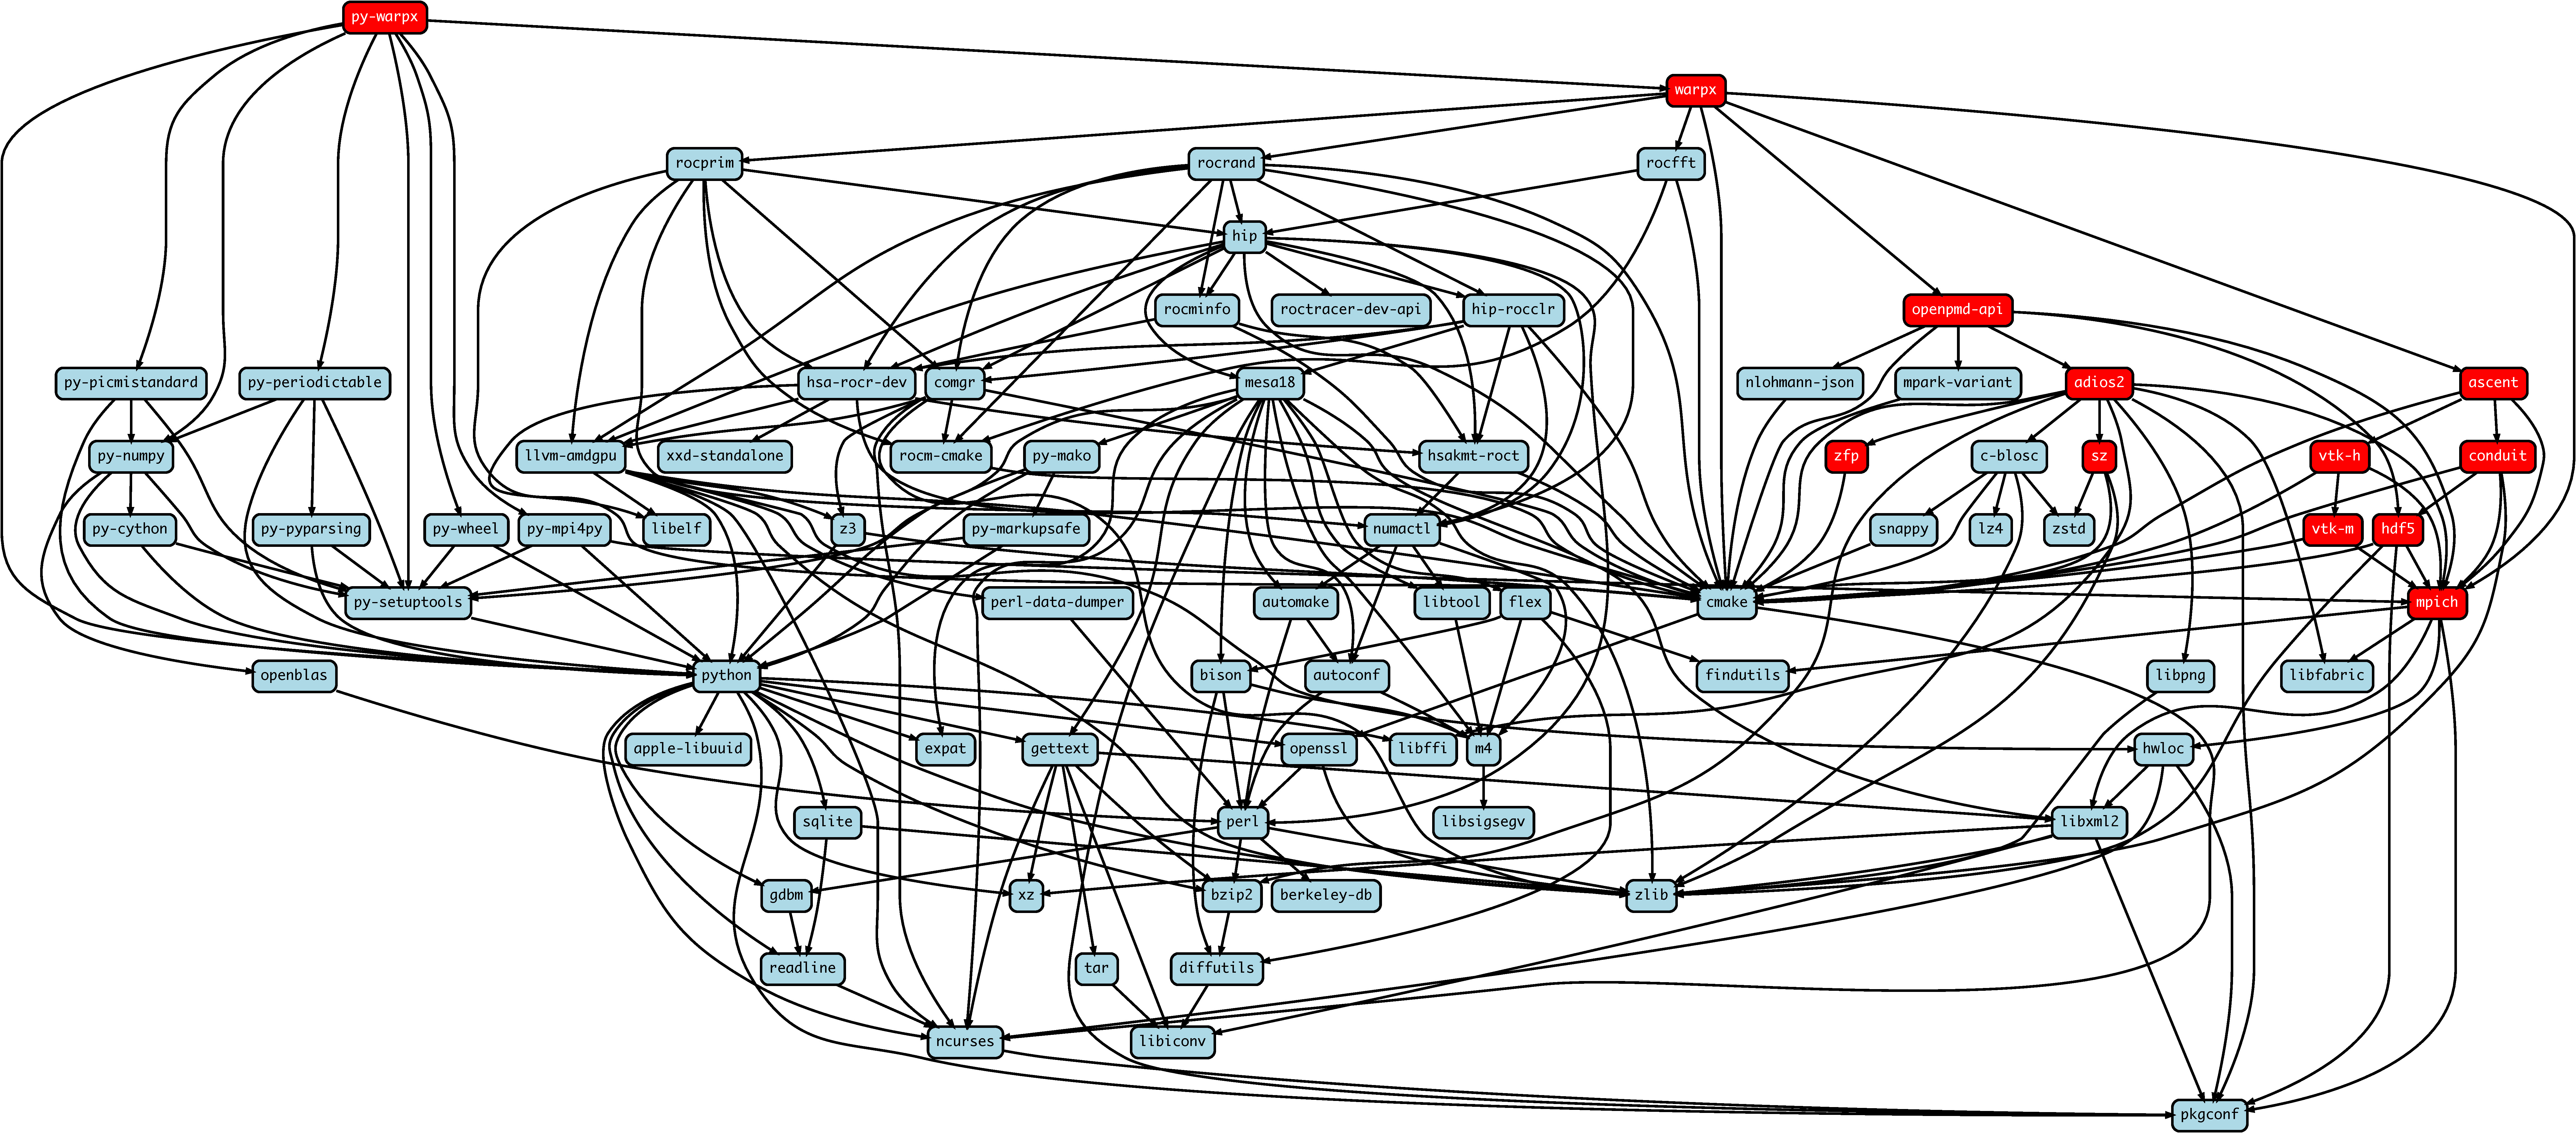
\includegraphics[width=.8\columnwidth]{figures/warpx.pdf}
%  \caption{ Dependencies of WarpX (built with AMD ROCm GPU support
%    enabled). E4S packages are shown in red.
%    \label{fig:warpx}
%  }
%\end{figure}

Managing dependencies for scientific software is notoriously
difficult~\cite{hoste+:pyhpc12,gamblin+:sc15,dubois2003johnny,hochstein+:2011-build}.
Scientific software is typically built from source to achieve good performance, and
configuring build systems, dependency versions, and compilers requires painstaking care.
In the past decade, the modularity of HPC software has increased due to well known
benefits such as separation of concerns, encapsulation, and code reuse. These enable
application codes to leverage fast math libraries~\cite{hypre,mfem,petsc,trilinos} and
GPU performance portability frameworks like RAJA~\cite{raja} and Kokkos~\cite{kokkos}.
However, the cost of modularity is integration complexity: consumers of components must
ensure that versions and other parameters are chosen correctly to ensure that all
integrated components work together.

{\it Package managers} emerged in the mid-1990's to mitigate the complexity of
integrating software packages in Linux distributions. In the past decade, their use has
exploded, particularly within language ecosystems like Python~\cite{pip},
Javascript~\cite{npm}, and Rust~\cite{cargo}, but also within the HPC community. The
HPC-centric package managers Spack~\cite{gamblin+:sc15} and
EasyBuild~\cite{hoste+:pyhpc12} are now widely used for software deployment at HPC
centers, and by developers and users installing their own software. The U.S. Exascale
Computing Project (ECP) has adopted Spack as the distribution tool for its
E4S~\cite{e4s} software stack (shown in Figure~\ref{fig:e4s-graph}), which contains
around 100 core software products and 500 required dependency packages.

\begin{figure*}
  \centering
  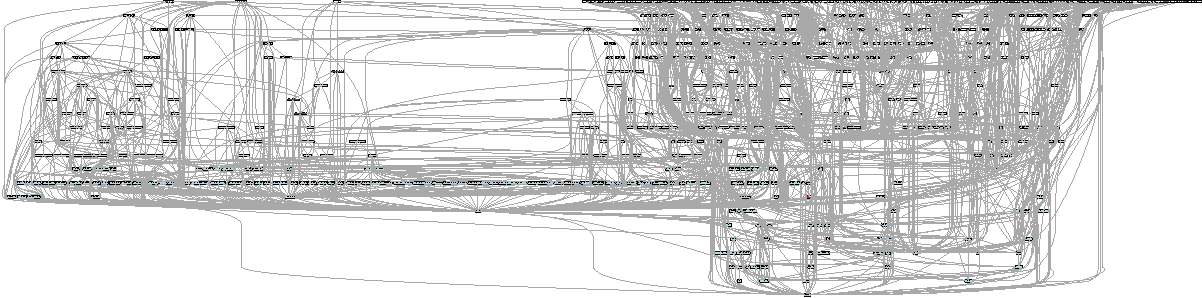
\includegraphics[width=\textwidth]{figures/e4s.pdf}
  \caption{
    Graph of package dependencies in the Extreme Scale Scientific Software Stack (E4S)~\cite{e4s}.
    Around 100 core software products are shown in red, and the 500 required dependencies
    are blue. The precise number of packages required for a deployment of E4S
    is system-specific, depending on platform and hardware (e.g., NVIDIA, AMD GPUs).
    \label{fig:e4s-graph}
  }
\end{figure*}

Package managers address the integration problem in two main ways. Systems like
EasyBuild and Nix~\cite{dolstra+:icfp08,dolstra+:lisa04} rely on human effort, where
maintainers develop fixed package configurations that define a common stack to be
shared among users. To deviate from the stack, users must update all configuration files
to ensure that versions and other parameters are consistent. More commonly, package
managers like Spack provide flexibility for the end user by incorporating {\it
  dependency solvers} at their core. Users can request arbitrary versions, and packages
declare {\it constraints} that bound the space of compatible configurations. The solver
selects a set of versions and configuration parameters that satisfy the user's
requirements and package constraints.

Dependency solving is NP-complete, even for a ``simple'' configuration space with only
packages and versions~\cite{dicosmo:edos,cox:version-sat}. Here, we focus on Spack's
dependency solver, known as the {\it concretizer}, which adds build options (variants),
compilers, target microarchitectures, and dependency versions to make the space even
larger. Most package managers use their own ad-hoc solver~\cite{abate2020dependency},
and Spack is no different; it has historically used its own {\it greedy} algorithm.
Heuristics were sufficient when there were only 245 packages~\cite{gamblin+:sc15}, but
now, Spack's mainline repository contains over 6,000 packages, each with many
constraints and options, and the original concretizer has begun to show its age. In
particular, it lacks:
\begin{itemize}
\item {\it Completeness}: in a growing number of cases, it may not find a solution even
  though one exists; and
\item {\it Optimality}: it provides no guarantees that it has found the ``best''
  of all valid solutions according to any criteria.
\end{itemize}

An increasing number of package managers use Boolean satisfiability (SAT) solvers to
resolve dependency constraints~\cite{abate2020dependency}, which works well for version
solving with a single optimization objective. With its added dimensions, Spack's solver
encodes a much larger configuration space {\it and} requires multi-objective
optimization. Encoding these semantics in pure SAT is {\it extremely} complex. Instead,
we have turned to Answer Set Programming
(ASP)~\cite{gebser+:asp-book,marek+:asp-origins}, a declarative model that allows us to
encode dependency semantics in a first-order, Prolog-like syntax. ASP solvers reduce
first-order logic programs to SAT and optimization, and they guarantee both complete
and optimal solutions. Unlike Prolog, they are also guaranteed to terminate. ASP
encodings are non-trivial, and this paper presents the first dependency solver capable
of making strong guarantees for the full generality of HPC dependency semantics.
Specifically, our contributions are:

\begin{enumerate}
\item A general mapping of Spack's DSL, compatibility semantics, and optimization rules
  to ASP;
\item A technique to optimize for reuse of existing builds in combinatorial package
  solves;
\item An ASP solver implementation in Spack that enables {\it complete} and {\it
  optimal} solutions; and
\item An evaluation of our system's performance on the E4S repository with tens of
  thousands of packages.
\end{enumerate}

Together, these contributions allow us to replace Spack's original concretizer with a
complete, optimizing solver, written in around 800 lines of declarative ASP. This
represents a leap forward in capability, maintainability, and extensibility to the
ever-increasing complexity of HPC software.

%-------------------------------------------------------------------------------
\section{Package Managers}
%-------------------------------------------------------------------------------
\label{sec:package-managers}

The idea of ``sofware release management'' for integrated sets of packages dates back to
a 1997 paper from Ven der Hoek et al.~\cite{van1997software}, and the first Linux
package managers emerged around the same time~\cite{rpm,apt}. Since then, the number and
complexity of software packages has grown enormously, as have the use cases for package
managers.

\subsection{Single-prefix Package Managers}

Package managers such as RPM, Yum, and APT~\cite{foster+:rpm03,silva:apt01,yum} are used
to manage the system packages of most Linux distributions. These tools focus on managing
one software stack, built with one compiler, which works well for system software and
drivers that underly all software on the system. They are designed so that software can
be upgraded in place for bugfixes and security updates. All software goes in to a single
{\it prefix}, e.g., {\tt /usr}, and for this reason, only one version of any package can
be installed at a time. Upgrades are prioritized over reproducibility, and users do not
have great flexibility over precise package versions and configurations.

Even in this limited package/version configuration space, dependency solving is
NP-complete~\cite{dicosmo:edos,mancinelli+:ase06-foss-distros} because any two
non-overlapping version constraints can cause a conflict. The Common Upgradeability
Description Format (CUDF) attempts to standardize an interface for external package
solvers~\cite{abate2012dependency,abate-2013-modular-package-manager} and has enabled
many encodings of the single-prefix upgrade problem: Mixed-Integer Linear Programming,
Boolean Optimization, and Answer Set
Programming~\cite{tucker+:icse07-opium,michel+:lococo2010,argelich+:lococo2010,gebser+:2011-aspcud}.
Most modern package solvers still use ad-hoc implementations instead of a common
external solver~\cite{abate2020dependency}.

\subsection{Language Package Managers}

Most modern language implementations also include their own package
managers~\cite{npm,pip,cargo,weizenbaum:pubgrub18}. The solver requirements for language
package managers are different from those in a linux distribution; they typically allow
multiple versions of the same package to be installed to support developer workflows and
reproducibility. Conflicts can arise, as most langauge module systems do not support
{\it linking} multiple versions of one package into a single executable. Javascript is a
notable exception to this. Language package managers still solve only for package
names and versions, ignoring compilers, build options, targets and other options that
expand the solution space. Most language package managers implement their own ad-hoc
solvers. Historically, these solvers were not complete, as
implementing a performant SAT solver in all but the lowest-level languages is quite
difficult. However, there has been a recent trend towards complete
solvers~\cite{pip-new-resolver,weizenbaum:pubgrub18} as complexity of language
ecosystems has grown. These systems do not support optimization beyond selecting recent
versions~\cite{abate2020dependency}.

\subsection{Functional and HPC Package Managers}

So-called ``functional'' package managers like
Nix~\cite{dolstra+:icfp08,dolstra+:lisa04} and Guix~\cite{courtes-guix-2015} allow users
to install arbitrarily many configurations of a given package. Like many HPC
deployments, they install each configuration to a unique prefix, but instead of a
human-readable name, they ensure that each installation gets a unique prefix by using a
hash of the bits of the installation itself. These systems do not use solvers to resolve
dependencies. Rather, they have very little conditional logic and rely on the specific
package recipes in a repository. As mentioned, Easybuild~\cite{hoste+:pyhpc12} is
similar in this regard, as it allows multiple configurations of packages by duplicating
package recipes and adhering to a strict naming convention to differentiate different
installations. In all of these systems, users must modify code in package recipes to
change the way dependencies are resolved.


%-------------------------------------------------------------------------------
\section{\spack}
\label{sec:software-model}
%-------------------------------------------------------------------------------
-- Greg
\subsection{Spec Syntax}

\subsection{Package DSL}

\subsection{Concretization}
- user configuration
- CLI arguments
- package constraints

\subsection{Dependency Model}
Discuss the software dependency model used in \spack and the future roadmap. Introduce concepts like variants, ABI compatibility etc. that are either implicit or disregarded by other package managers.


%-------------------------------------------------------------------------------
\section{Answer Set Programming}
%-------------------------------------------------------------------------------
-- Todd
Background on ASP solvers

%-------------------------------------------------------------------------------
\section{Modeling Software Dependencies with ASP}
%-------------------------------------------------------------------------------
\label{sec:asp-model}
At a high-level, with the introduction of \clingo, each concretization
combines:
\begin{enumerate}
\item A large number of \emph{facts} characterizing the specific problem being solved
\item A small \emph{logic program} encoding the rules and constraints of the software model
\end{enumerate}
The facts are always generated starting from one or more 
\emph{root specs} that need to be concretized, and they account 
for both the metadata contained in package recipes and the 
current state of \spack{} in terms of configuration and 
installed software.
For instance, a simple directive such as:
\begin{minted}[fontsize=\small, bgcolor=bg]{python}
version('1.2.11', sha256='ah45rstgef...')
\end{minted}
in \texttt{zlib}'s recipe is translated to the following fact:
\begin{minted}[fontsize=\small, bgcolor=bg]{text}
version_declared("zlib", "1.2.11", 0, "package_py").
\end{minted}
in our ASP solve. Similarly, the request to concretize
\begin{minted}[fontsize=\small, bgcolor=bg]{text}
zlib@1.2.11
\end{minted}
generates the following three facts:
\begin{minted}[fontsize=\small, bgcolor=bg]{text}
root("zlib").
node("zlib").
version_satisfies("zlib","1.2.11").
\end{minted}
stating that \texttt{zlib} is a root node and should satisfy
a version requirement.
A typical solve has around $10k-100k$ facts which include
the encoding of dependencies, variants, preferences, etc.

The logic program encodes the software model used by \spack{}
and is solely composed by first-order rules, integrity 
constraints and optimization objectives. 
The declarative nature of ASP makes it easy to enforce 
certain properties on the optimal solution. For instance, 
these three lines ensure that we never have a cyclic dependency
in a DAG:
\begin{minted}[fontsize=\small, bgcolor=bg]{text}
path(A, B) :- depends_on(A, B).
path(A, C) :- path(A, B), depends_on(B, C).
:- path(A, B), path(B, A).
\end{minted}
The first rule establishes the base case: if \texttt{A} depends
on \texttt{B} there is a path from \texttt{A} to \texttt{B}.
The second rule defines paths to transitive dependencies 
with a recursive definition: if there is a path from \texttt{A} 
to \texttt{B} and \texttt{B} depends on \texttt{C}, there is
a path from \texttt{A} to \texttt{C}. The final line is an 
\emph{integrity constraints} stating that paths from \texttt{A} 
to \texttt{B} and paths from \texttt{B} to \texttt{A} cannot 
occur at the same time in a valid solution.

To give a rough idea of the compactness and expressiveness of 
the ASP encoding, the entire logic program for the software 
model described in Section~\ref{sec:software-model} is around 
$500$ lines of code. The concretization process is straightforward
to follow conceptually within \spack:
\begin{enumerate}
\item Facts are generated for the current concretization \footnotemark
\item The logic program and the facts are sent to the solver
\item The concretized DAG is rebuilt from the \emph{optimal} result
\end{enumerate}
\footnotetext{It's worth stressing that the logic program changes only
when the underlying software model changes, as opposed 
to the generated facts that are different whenever the root
spec to be concretized or \spack's configuration changes.}
The word ``optimal'' is emphasized since, while rules and integrity 
constraints fully determine if a solution is valid, we need 
optimization targets to select one of the many possible solutions
in a way that fits user's expectations.

A good example to illustrate this point is target selection for DAG nodes.
In \spack{} each node being built has a target microarchitecture associated with it, and we want to use the best target possible while respecting the constraints coming from the compiler (some compilers don't support generating code for some targets) and from the configuration. 
Previously this required some complicated logic mixed with the rest of the solve.
The introduction of \clingo{} simplified the problem definition by a great amount. A cardinality constraint is used to express that each node must have one and only one target:
\begin{minted}[fontsize=\small, bgcolor=bg]{text}
1 { node_target(Package, Target) : 
    target(Target) } 1 :- node(Package).
\end{minted}
A rule ensures that the user's choice to set the target to a specific value is respected:
\begin{minted}[fontsize=\small, bgcolor=bg]{text}
node_target(P, T) :- node(P), node_target_set(P, T).
\end{minted}
An integrity constraints prevents to choose a target not supported by the current compiler:
\begin{minted}[fontsize=\small, bgcolor=bg]{text}
:- node_target(P, T),
   not compiler_supports_target(C, V, T),
   node_compiler(P, C),
   node_compiler_version(P, C, V).
\end{minted}
These three statements fully describe the characteristics of a valid solution. To pick the \emph{optimal} solution we also \emph{weight} the possible targets
(the lower the weight, the best the target) and optimize over the sum of target weights:
\begin{minted}[fontsize=\small, bgcolor=bg]{text}
node_target_weight(P, W) :- 
  node(P), node_target(P, T), target_weight(T, W).
#minimize { W@5,P : node_target_weight(P, W) }.
\end{minted}

\subsection{Generalized Condition Handling}
A peculiar feature of \spack, as a package manager, is that it doesn't only optimize for versions but for many other aspects of the build as well e.g. which compiler to use, which microarchitecture to target, etc. 
The DSL used for package recipes reflects this complexity by having multiple directives to declare different properties or constraints for each software, as seen in Section~REFMISSING. 

One interesting abstraction, that we observed while coding the ASP logic program, is that each of these directives can be seen as a way to impose additional constraints on the solution, conditional on other constraints 
being met. For instance, the following directive in a package:
\begin{minted}[fontsize=\small, bgcolor=bg]{python}
depends_on('hdf5+mpi', when='+mpi')
\end{minted}
means that, if the spec has the \texttt{mpi} variant turned on, then it depends on \texttt{hdf5+mpi}. Similarly:
\begin{minted}[fontsize=\small, bgcolor=bg]{python}
provides('lapack', when='@12.0:')
\end{minted}
means that a package provides the \texttt{LAPACK} API starting at version $12.0$.
This property allowed to encode all the directives as \emph{generalized conditions}, where most of the sematics is encoded abstractly in a few lines of the logic program.

Getting back to a simple example, the snippet below:
\begin{minted}[fontsize=\small, bgcolor=bg]{python}
class H5utils(AutotoolsPackage):
    depends_on('png@1.6.0:', when='+png')
\end{minted}
is mapped to the following facts for the solver:
\begin{minted}[fontsize=\small, bgcolor=bg]{text}
condition(153)
condition_requirement(153, "node", "h5utils")
condition_requirement(
  153, "variant_value", "h5utils", "png", "True"
)
imposed_constraint(
  153, "version_satisfies", "libpng", "1.6.0:"
)
dependency_condition(153, "h5utils", "libpng")
\end{minted}
It's straightforward to see that:
\begin{itemize}
\item Each directive is associated with a unique global ID.
\item Constraints are either ``requirement'' or ``imposed''. 
\item Different type of conditions have different semantics\footnotemark
\end{itemize}
\footnotetext{For instance, the \texttt{dependency\_condition} fact is present only for \texttt{depends\_on} directives and activates logic that is specific to dependencies.}
The code to trigger and impose general conditions in the logic program is surprisingly simple to read. ASP conditional rules allow us to effectively build new rules from input facts:
\begin{minted}[fontsize=\small, bgcolor=bg]{text}
condition_holds(ID) :-
condition(ID);
attr(N, A1): condition_requirement(ID, N, A1);
attr(N, A1, A2): condition_requirement(ID, N, A1, A2);
...
\end{minted}
based on their \emph{arity}. Other rules, similar to:
\begin{minted}[fontsize=\small, bgcolor=bg]{text}
attr(N, A1) :- 
  condition_holds(ID), imposed_constraint(ID, N, A1).
\end{minted}
enforce the imposed constraints when a condition holds.

\subsection{Example: Specialize LAPACK Providers}
\subsection{Example: CUDA/RoCM Conditional Variants}




\section{Reusing already built packages}
\label{sec:reuse}
%-------------------------------------------------------------------------------
\section{Reusing Already Built Packages}
%-------------------------------------------------------------------------------
\label{sec:reuse}

While \spack{} is primarily a package manager installing software \emph{from sources},
the ability to reuse already built software and mix it seamlessly with source builds has
been a critical request from the community for several years.

\begin{figure}[htb]
  \centering
  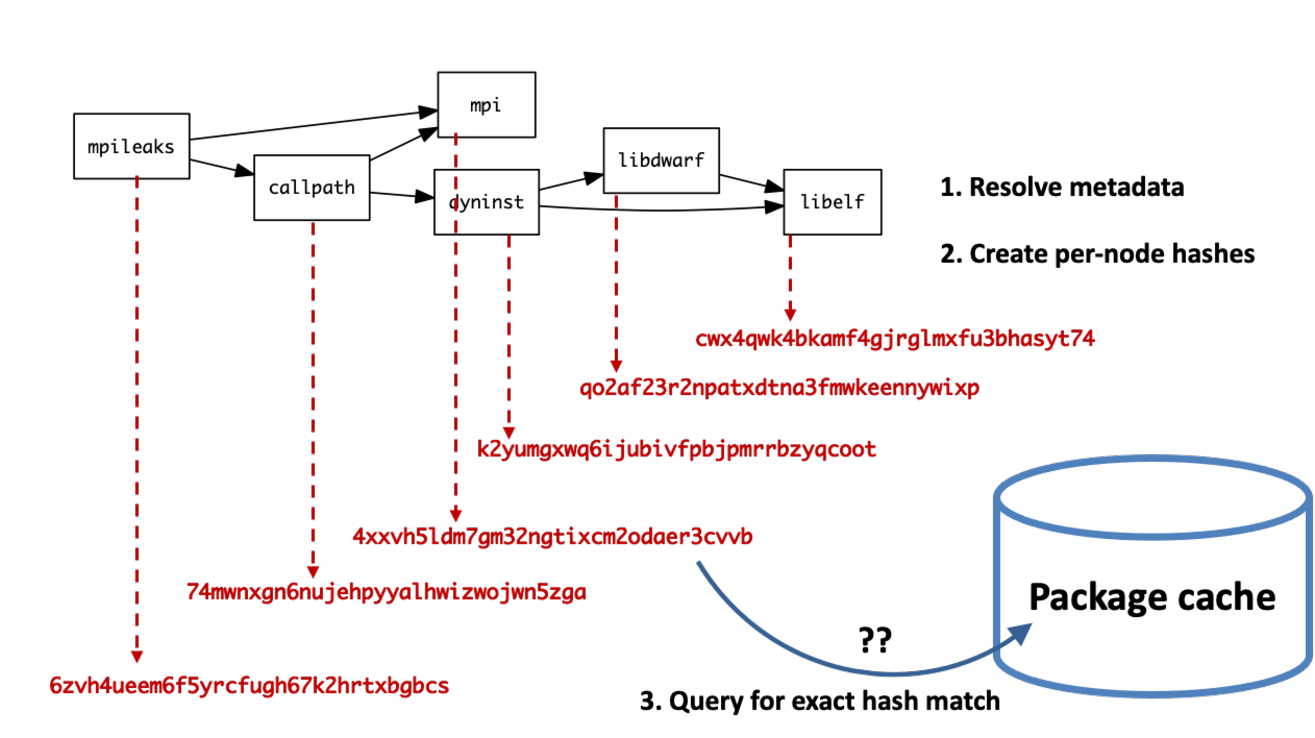
\includegraphics[width=.8\columnwidth]{figures/hash-cache.pdf}
  \caption{Hash-based reuse in the original \spack concretizer}
  \label{fig:hash_reuse}
\end{figure}

Functional packaging systems, including \spack{} with the old concretizer, reuse builds
via metadata hashes. This mechanism relies on the fact that, when an installation graph
is concretized, each node in the DAG is given a unique hash, as shown in
Figure~\ref{fig:hash_reuse}.
%A user can then query for an exact hash match to reuse
%something that is either already installed or available as a binary package.
Unless the user was explicit, \spack{} only reused packages if their hashes matched
exactly. Small configuration changes easily result in little or no reuse.

%The issue with this way of proceeding is that users are \emph{effectively
%overconstraining} their request since specifying the hash is equivalent to specifying
%\emph{all the metadata} of the associated spec. This exposes users to need frequent
%changes in their configuration, since hashes are very sensitive to small changes, and
%prevents them from finding other satisfying specs that might be available.
% FIXME: expand on Nix, Guix, Conan etc. ?

%\subsection{Optimizing for Software Reuse}

A more effective way to approach software reuse can be achieved by leveraging the
``Generalized Condition Handling'' logic described in
Section~\ref{subsec:generalizedcond}. First, all the metadata from installed packages
can be encoded into facts:
\begin{minted}[fontsize=\tiny, bgcolor=bg]{prolog}
installed_hash("zlib","7fatdw6gth5nlfdj4d463rdhrby6qvx3").
imposed_constraint("7fatdw6gth5nlfdj4d463rdhrby6qvx3","node","zlib").
imposed_constraint("7fatdw6gth5nlfdj4d463rdhrby6qvx3","version","zlib","1.2.11").
imposed_constraint("7fatdw6gth5nlfdj4d463rdhrby6qvx3","node_platform","zlib","linux").
imposed_constraint("7fatdw6gth5nlfdj4d463rdhrby6qvx3","node_os","zlib","ubuntu20.04").
imposed_constraint("7fatdw6gth5nlfdj4d463rdhrby6qvx3","node_target","zlib","icelake").
...
\end{minted}
The encoding is based on \texttt{imposed\_constraint}, but the constraint ID is the
hash associated with the installed package. To minimize the number of builds from
source, the solver is allowed to choose a hash to resolve any package:
\begin{minted}[fontsize=\small, bgcolor=bg]{prolog}
{ hash(P, Hash) : installed_hash(P, Hash) } 1
 :- node(P).
\end{minted}
Impose all constraints associated with chosen hashes:
\begin{minted}[fontsize=\small, bgcolor=bg]{prolog}
impose(Hash) :- hash(P, Hash).
\end{minted}
And number of builds (packages \emph{without} a hash) is minimized:
\begin{minted}[fontsize=\small, bgcolor=bg]{prolog}
build(P) :- not hash(P, _), node(P).
#minimize { 1@100,P : build(P) }.
\end{minted}

This is a remarkably simple encoding for a complex constraint problem that cannot be
solved with the prior greedy concretizer. However, the devil is in the details.
Minimizing builds can have two effects---it can cause the concretizer to prefer an
existing installation over building a new version of a package, but if set as the
highest optimization priority, it also causes the concretizer to configure newly built
packages in any way that {\it minimizes dependencies}. Generally, though, users expect
new builds to use regular defaults---i.e., most recent version, preferred variants, etc.
As an illustrative example, building \texttt{cmake} with these objectives will build
{\it without} without networking capabilities, because it omits \texttt{openssl} and its
dependencies from the graph!

%The
%trickiest point is how to choose at which priority the minimization of builds should be
%put in our multi-objective optimization criteria. The difficulty we face here stems from
%the different nature that an already built configuration has with respect to one that we
%still have to build. In the former case we can't change any aspect of the underlying
%graph, e.g. we can't choose a different version or a different set of variants to
%improve some optimization score, since the installed configuration is immutable. In the
%latter case instead, since we still have to build the software, we would like to choose
%the most recent version, use the preferred variants etc.

%% Reasoning on this issue it becomes evident that having a single optimization criteria
%% that accounts for both installed and non-installed software would always lead to
%% unsatisfying behavior. For instance, if we optimized for minimizing builds at the
%% highest priority and have no installed software to reuse, the solver would choose
%% minimal DAGs even though that means using old versions or non-default values for
%% variants. If a user asked to build e.g. \texttt{cmake} it would probably be unexpected
%% to build one version without networking capabilities just because that permits to trim
%% \texttt{openssl} and its dependencies from the graph!

Our solution is to split the optimization criteria into two identical ``buckets'', one
for installed software and one for software that is yet to be built, and optimize for
them at different priorities:
\begin{enumerate}
\item Minimize all objectives for software to be built
\item Then, minimize the number of builds
\item Minimize the objectives for already built software
\end{enumerate}
Minimizing the number of builds at a priority that is always higher than any other
criteria for installed software, but always lower than any criteria for software to be
built allows \spack{} to pick the best version available from what is installed without
adversely affecting the choice of defaults for built packages. This is actually simple
to encode in ASP:

\begin{minted}[fontsize=\footnotesize, bgcolor=bg]{prolog}
build_priority(P, 200) :- build(P), node(P).
build_priority(P, 0)   :- not build(P), node(P).
% ....
#minimize{
    W@5+Priority,P
    : version_weight(P, W), build_priority(P, Priority)
}.
\end{minted}

Here, {\tt Priority} will be 200 for built packages and 0 for preinstalled packages, and
we can use this to control the priority of the minimization objective. This {\tt
  \#minimize} sums into {\it two} buckets in a global per-solution vector, which is
ultimately compared lexicographically.
%
%To conclude this section we will show an example of how effective this approch is to
%reuse software.
%
Figure~\ref{fig:noreuse} shows a concretization relying on purely hash-based software
reuse. We can see that no match was found and 20 installations need to be performed from
source. In Figure~\ref{fig:reuse} we show the same concretization with the reuse logic
turned on. In this case 16 installed packages can be reused and only 4 need to be built.
Note that reuse takes priority over the defaults for already installed software,
allowing \spack{} to reuse \texttt{cmake} 3.21.1 even though the preferred version for a
new build is 3.21.4.

\begin{figure}[h]
  \centering
  \subfloat[][With hash-based reuse: all misses]{
    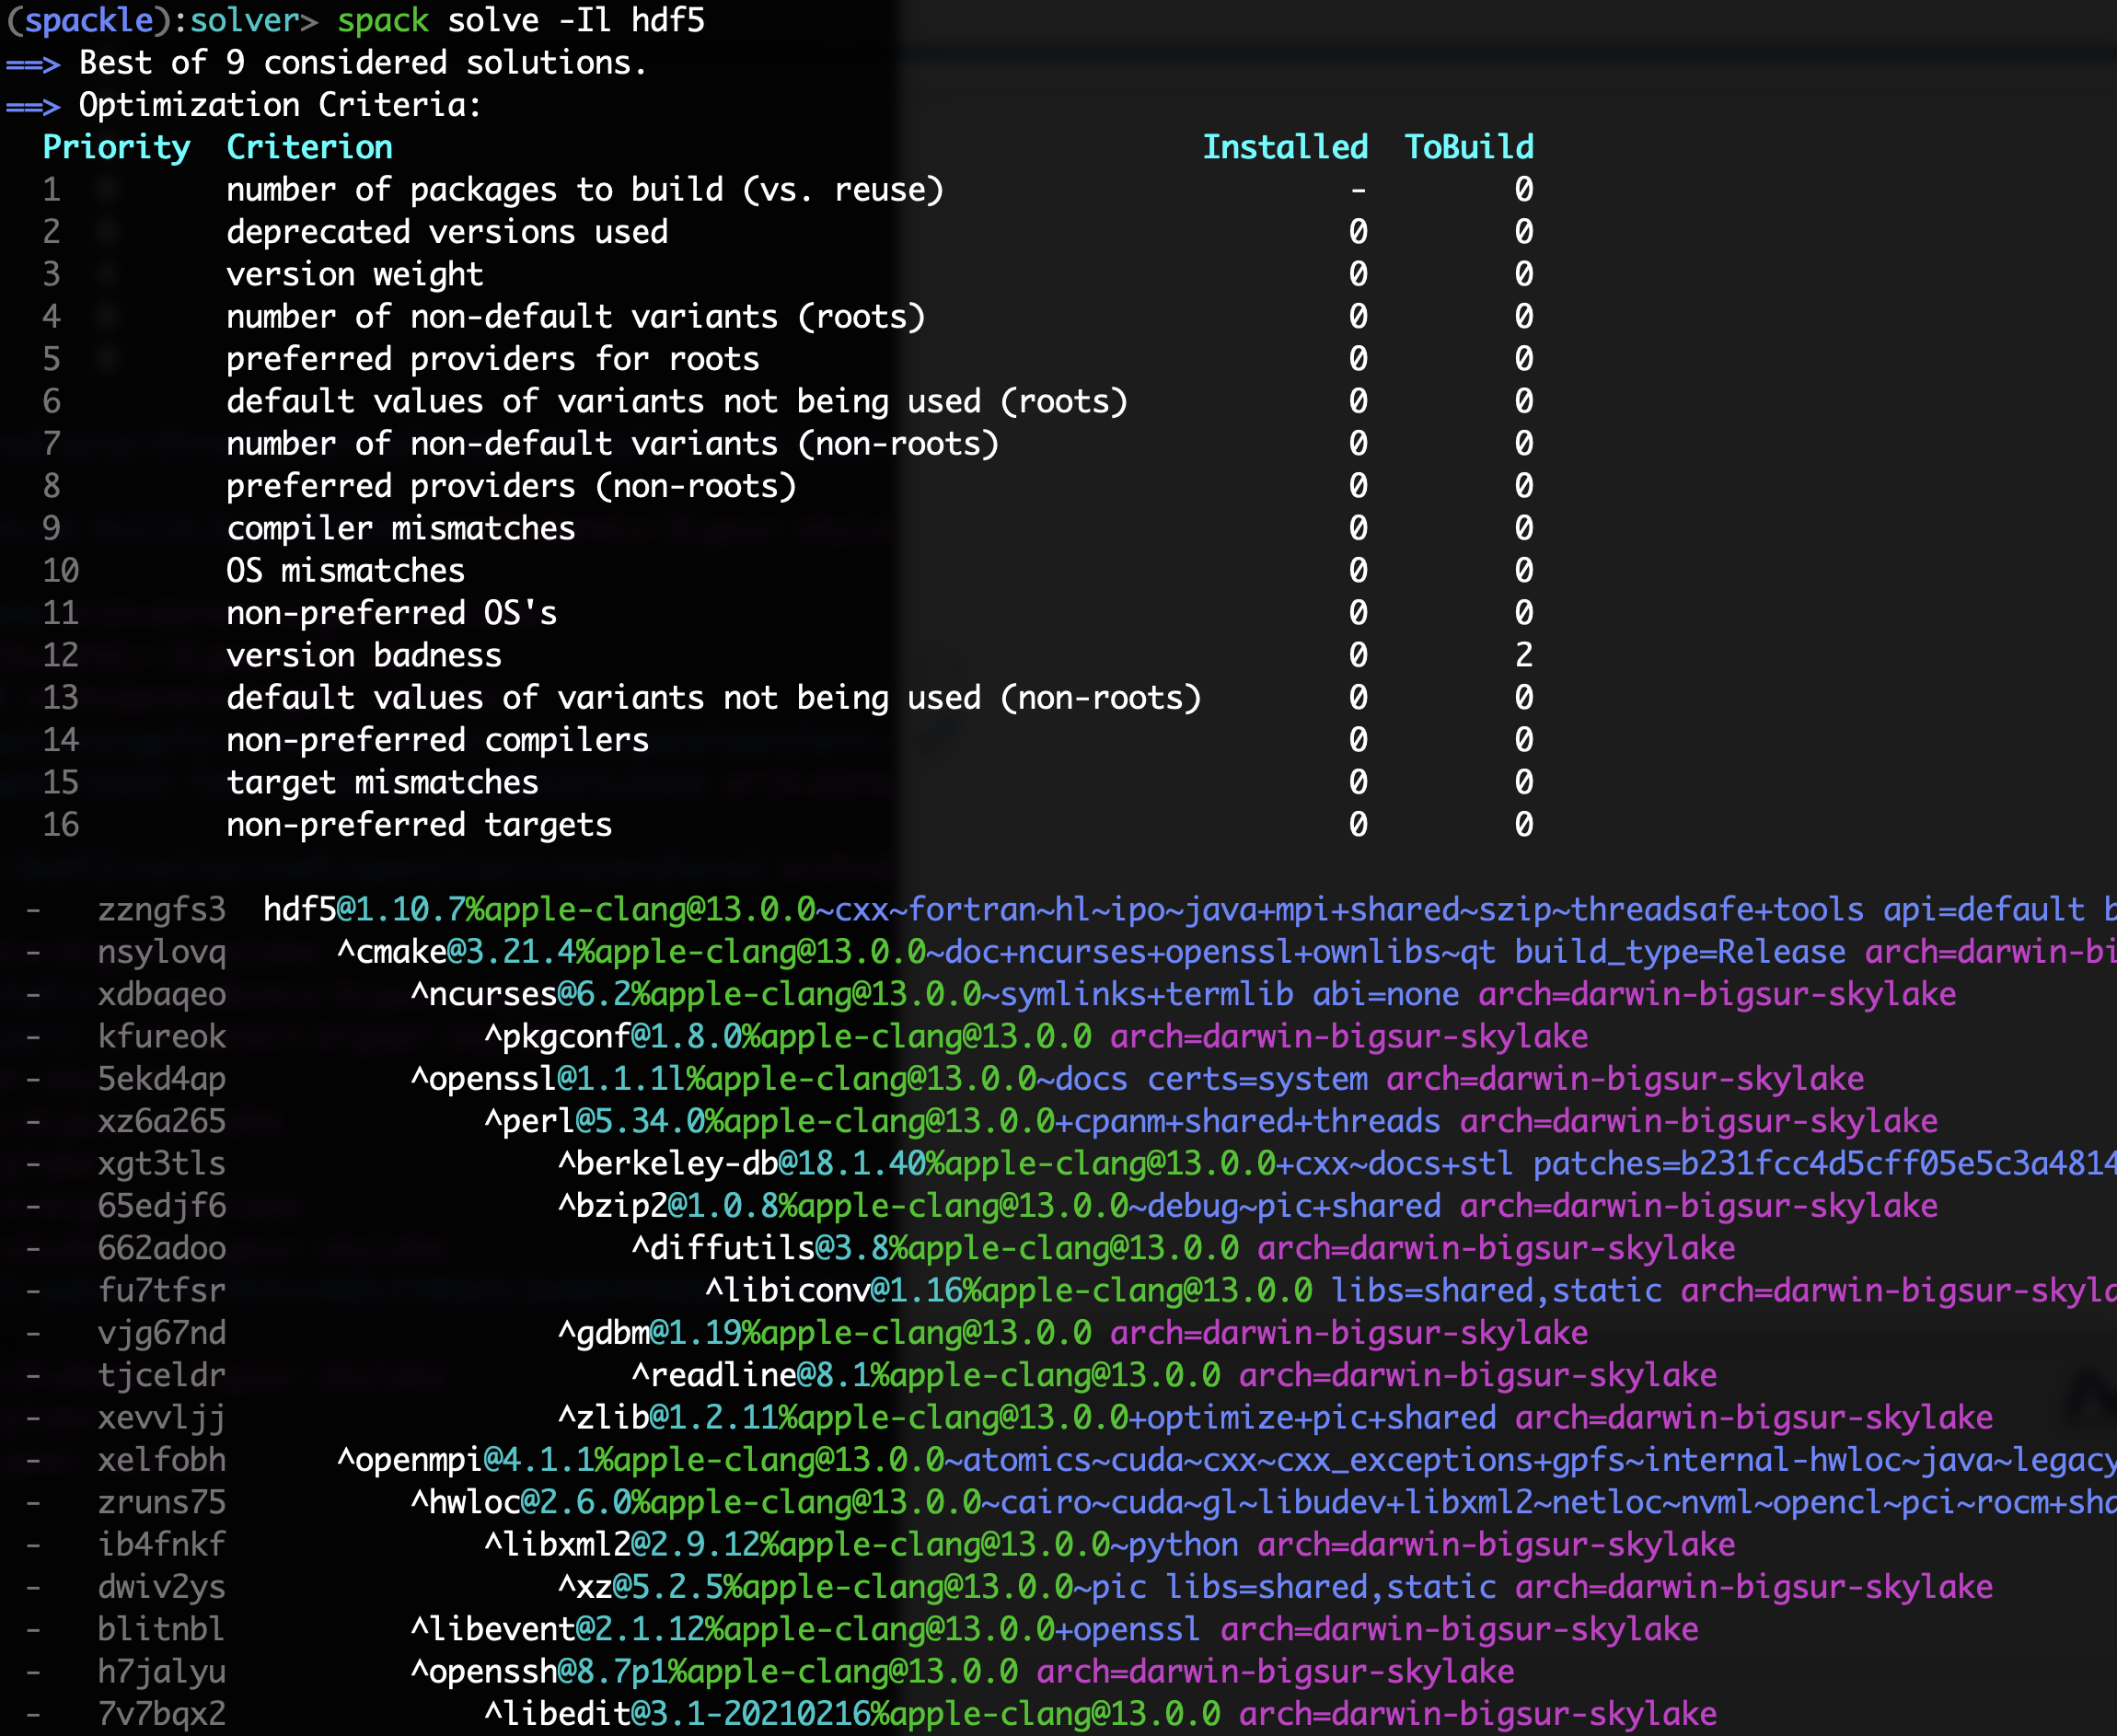
\includegraphics[width=2.4in]{figures/no-reuse.png}
    \label{fig:noreuse}
  }\\
%  \caption{Concretization of \texttt{hdf5} with pure hash-based reuse: all misses}
%\end{figure}
  %\begin{figure}[h]
  \subfloat[][Solving for reuse: 16 packages are actually acceptable]{
    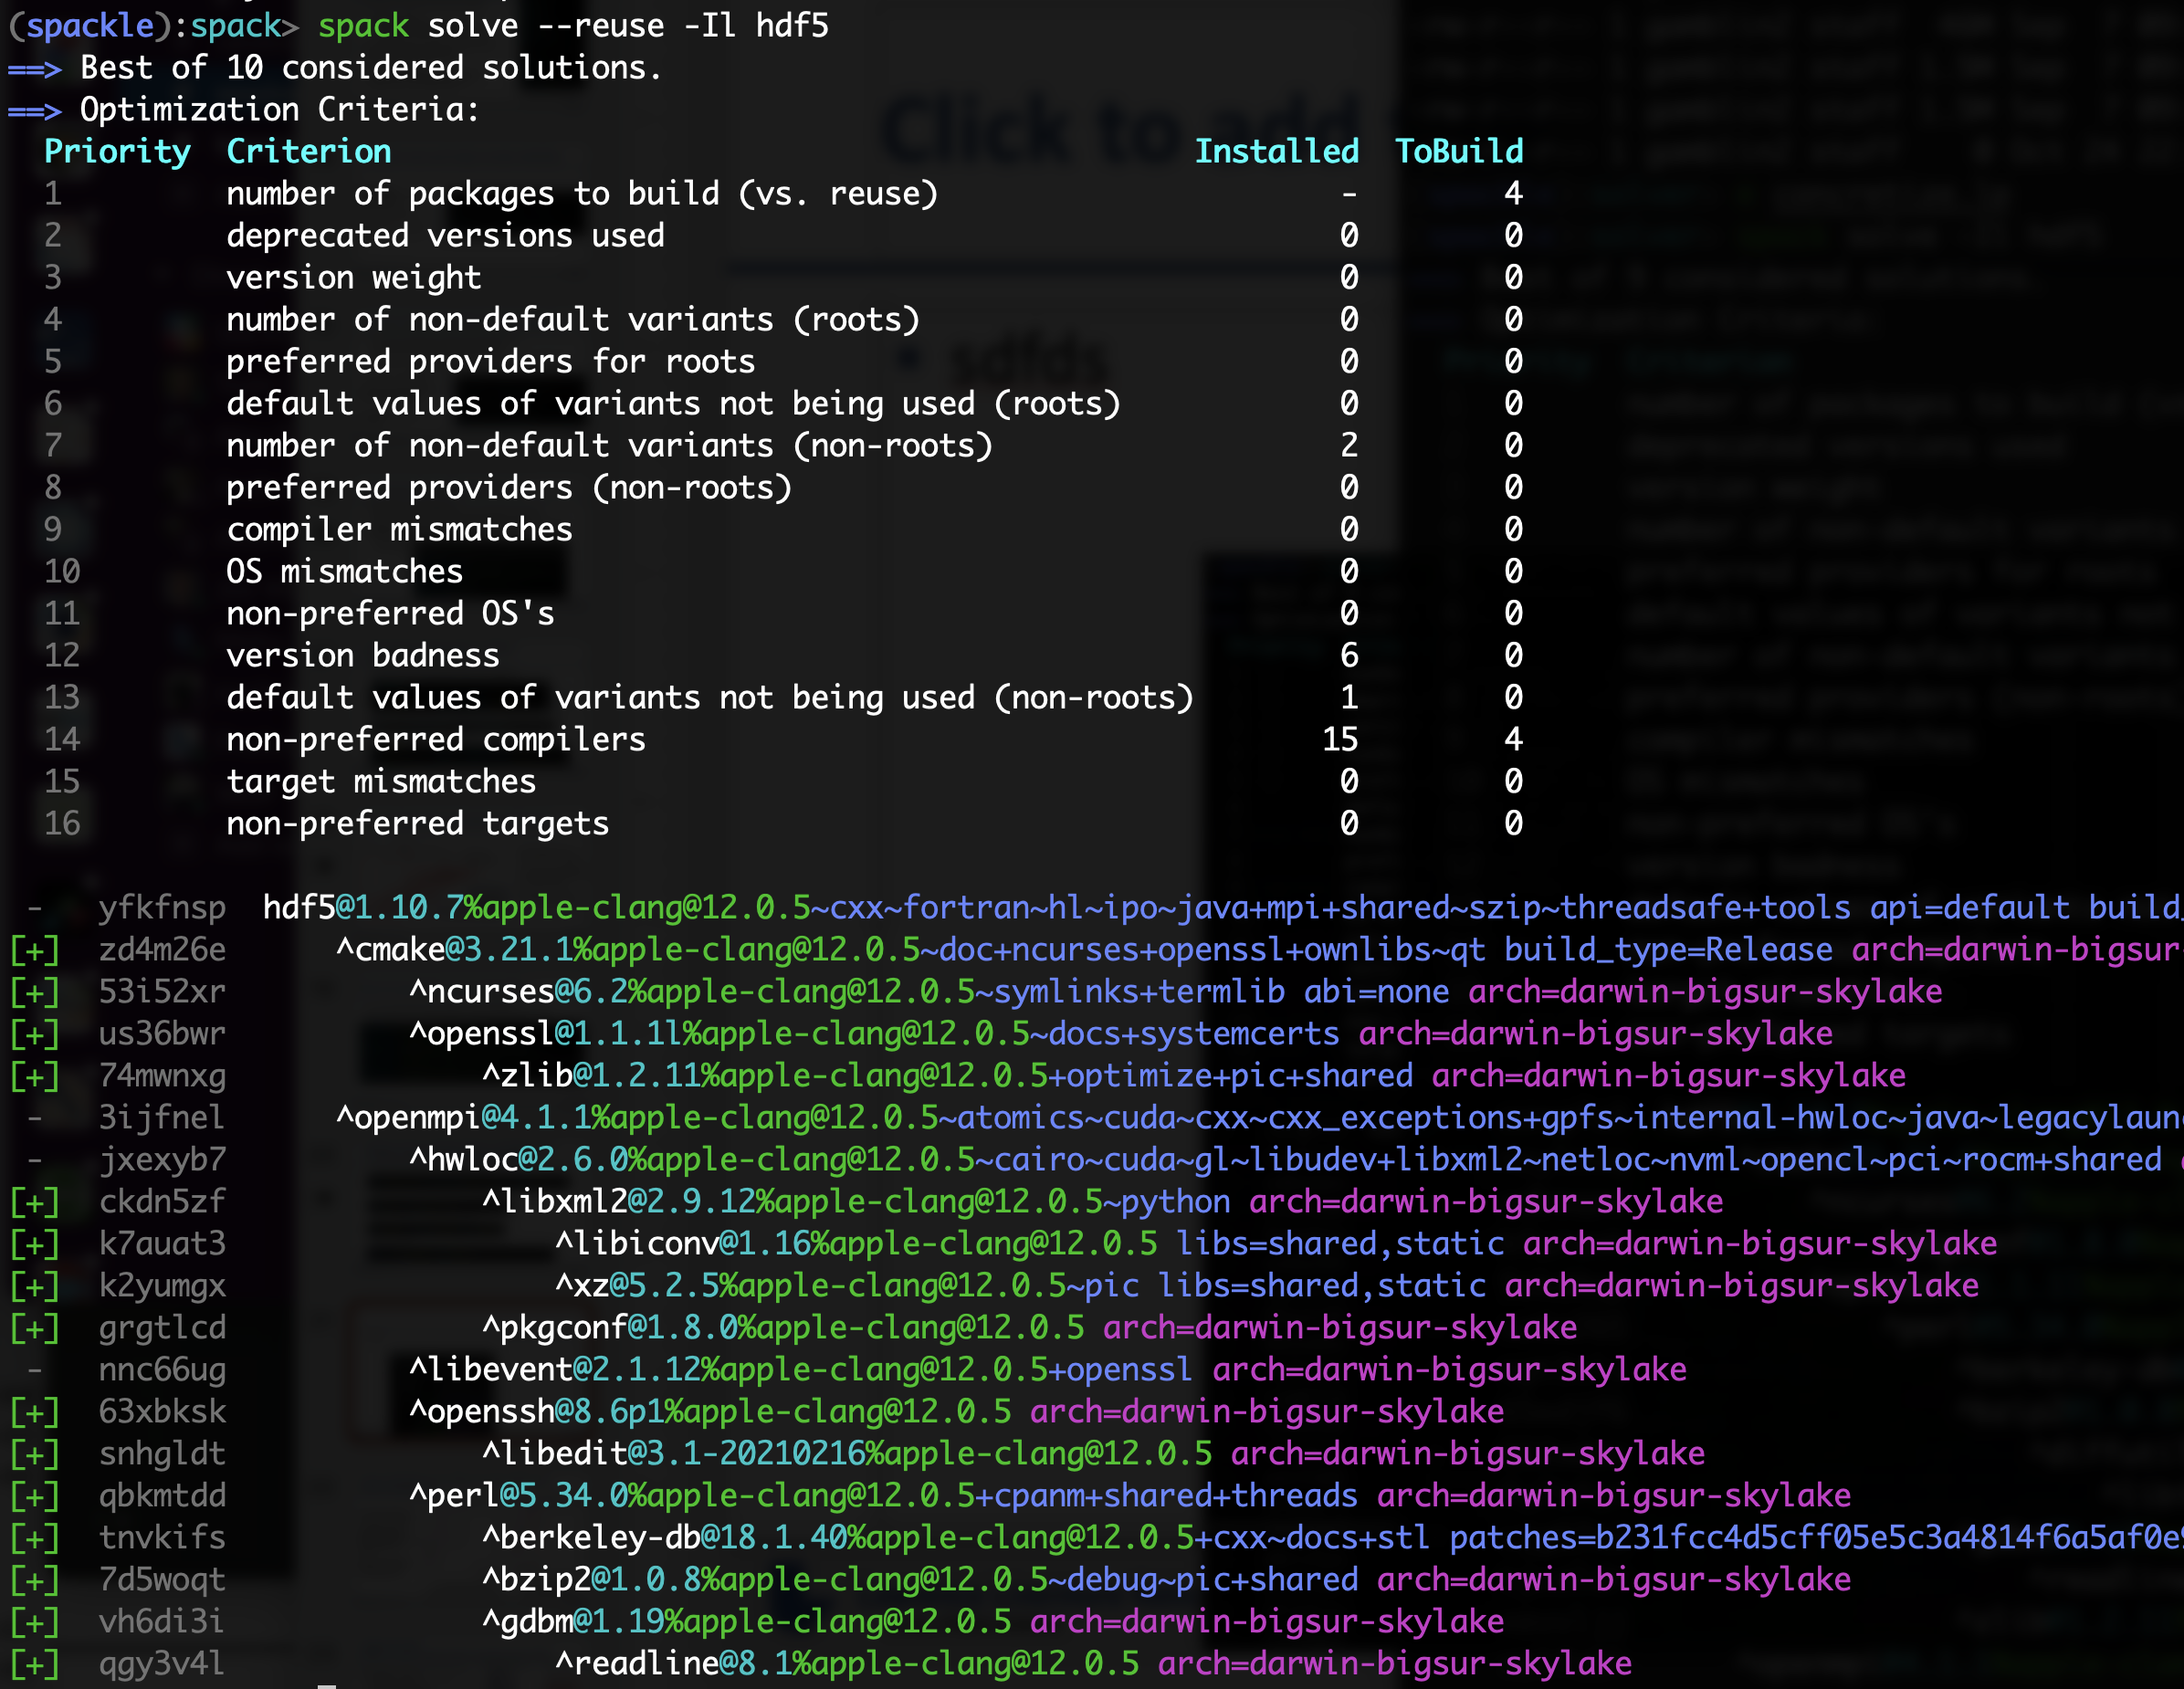
\includegraphics[width=2.4in]{figures/reuse.png}
    \label{fig:reuse}
  }
  \caption{Concretization with and without reuse optimization.}
  %\caption{The solver is asked to concretize \texttt{hdf5} trying to reuse installed software as much as possible. We see that 16 installed packages are actually acceptable to be reused. Another notable take is that, due to the priority chosen for minimizing the number of builds it is actually acceptable to \emph{reuse} \texttt{cmake} at version 3.21.1 even though the preferred version if it was to be built is 3.21.4}

\end{figure}


%- reuse of half the generalized condition
%- Reusing built dependencies
%- architecting optimization criteria for builds vs. reuse


%-------------------------------------------------------------------------------
\section{Error Handling for Unsolvable Problems}
%-------------------------------------------------------------------------------
\label{sec:error-handling}
%-------------------------------------------------------------------------------
\section{Error Handling for Unsolvable Problems}
%-------------------------------------------------------------------------------
\label{sec:error-handling}

Generating useful debug messages and error output from logic solvers can be challenging.
Solvers algorithms are sufficiently complex that an ``unsatisfiable'' end-state sometimes cannot be easily mapped to particular offending constraints.
One common method for error messages in solvers are subset-minimal unsatisfiable cores.
Subset-minimal unsatisfiable cores are unsatisfiable subsets of solution for which removing any element from the overall problem results in a satisfiable problem.
In a nearly trivial case, the clingo program

\begin{minted}[fontsize=\small, bgcolor=bg]{prolog}
foo(x)
foo(y)

:- foo(A), foo(B), A != B.
\end{minted}

will yield a subset-minimal unsatisfiable core of

$$ {foo(x), foo(y)} $$

assuming it is configured appropriately to allow each fact in the core.

Configuring clingo to generate subset-minimal unsatisfiable cores is non-trivial.
Clingo only generates unsatisfiable cores when using the ``usc'' optimization strategy.
It also does not naturally generate subset-minimal unsatisfiable cores; the unsatisfiable core returned by clingo can be quite large.
Mitigating the size of the cores, clingo cores only contain facts that are presented to the solver as ``assumptions'' and allowed as choice points for the algorithm.
Including the assumptions as choice points in the algorithm means that there is a trade-off between the comprehensiveness of the generated cores and the runtime of the program, as increased choice leads directly to increased runtime.

Generating a subset-minimal core from the non-minimal cores generated by clingo is possible.
It requires iterative solves for each element of the core, which can be prohibitive for larger core sizes.
The algorithm is in pythonic psuedocode below.

\begin{minted}[fontsize=\small, bgcolor=bg]{text}
solution, core = solve(assumptions=assumptions)

if core:
    min_core = core[:]
    for fact in core:
        min_core.remove(fact)
        solution, core = solve(
        if solution:
            min_core.append(fact)

    raise UnsatisfiableError(min_core)
...
\end{minted}

This algorithm can be very slow.
Iterative solves are not as expensive as the initial solve, potentially by an order of magnitude, but core sizes can be very large

Using a naive approach in which every fact from the program is an assumption in clingo, simple \spack{} problems like concretizing ``hwloc'' can generate cores with over 30,000 elements.
In one case we tested, over 30,000 elements were generated for a core when the subset-minimal core contained just two elements.
Minimizing cores of this size is infeasible, with minimization times over 40 minutes for a problem that solves in tens of seconds.

An additional weakness of the naive approach is that rules in clingo cannot be assumptions.
Therefore the subset-minimal unsatisfiable core is a collection of facts, with no information about which integrity constraints of the problem are violated by those facts.
That information can be difficult to glean without expert knowledge.

In response to those weaknesses of the naive approach, we devised a more lightweight approach for \spack.
We added a function to our clingo program with the signature \texttt{error/1.}.
Every integrity constraint in the concretizer program contains a term that is \texttt{error(msg)}, where ``msg'' is a string describing the purpose of the integrity constraint.
The error terms are the only facts in the program which are given as constraints to clingo.
This leads to unsatisfiable cores small enough to be minimized in a reasonable time \textemdash there are 16 assumptions in the program, which is the worst-case for the iterative solves necessary for core minimization.
In practice, this can be done in a small fraction of the original solve time.
Satisfiable solves for the ``hwloc'' package take on the order of ten seconds, and core minimization adds around another second.
Performance numbers will be discussed in more detail in the ``Performance Results'' section.

Future work will revolve around how much of the detail of the naive approach can be reintegrated with the error messages without degrading performance.
This will include work on batching tests in the minimization algorithm.
Because clingo's unsatisfiable cores tend to be very large compared to the subset-minimal cores for this problem, we may be able to drastically reduce the number of necessary tests by attempting to remove some fraction of the entire core at once, only testing in smaller granularity when we encounter a portion of the core containing an element of the minimal subset.



%-------------------------------------------------------------------------------
\section{Performance Results}
%-------------------------------------------------------------------------------
\label{sec:perf-results}
%-------------------------------------------------------------------------------
\section{Performance Results}
%-------------------------------------------------------------------------------
\label{sec:perf-results}

% How is the ASP based solver performing?

The \clingo{} solver performance given a logic program depends on a number of factors. First, the number of facts in a specific concretization. Second, the configuration and various optimization parameters passed to the solver.

The solving process consists of four stages: \emph{setup}, \emph{load}, \emph{ground}, and \emph{solve}. The first two are preliminary phases and the other two perform the actual solve. Specifically, the setup phase generates the facts for the given spec, whereas the load phase loads the main logic program (i.e., the rules of the software model) as a resource into the solver. The grounding phase is the first part of the actual solve, it turns the facts and first-order logic rules into propositional logic. Once we have a grounded program, we can run the last phase, which is the full solve in \clingo{}.

We instrumented the solving code such that we obtained time measurements for each of the phases and the total time for the whole process.

\subsection{System Setup}

All performance runs were executed on a single node each of the Quartz
and Lassen supercomputers at Lawrence Livermore National
Laboratory. Each node of Quartz is an Intel Haswell CPU with 128GB of
memory. Each node of Lassen is an IBM Power9 little-endian CPU with
256GB of memory. No hardware accellerators were used in any of our
testing. All code ran out of an NFS directory running NFSv3.

\subsection{Solve timings for all packages}

In this section we examine the solving times for all the packages. First, we focus on the relation between the solving times and the number of dependencies for each package.

For number of dependencies, we measured the number of possible
dependencies added to the solve, rather than the total dependencies in
the result, because it is a closer measure of the necessary work for
the solver. This leads to natural clustering in the number of
dependencies, as many simple dependencies lead to large numbers of
potential dependencies that dwarf other differences between specs.


\begin{figure*}[htb]

    \centering
    \subfloat[][Ground times]{
    \label{subfig:deps_quartz_load}
        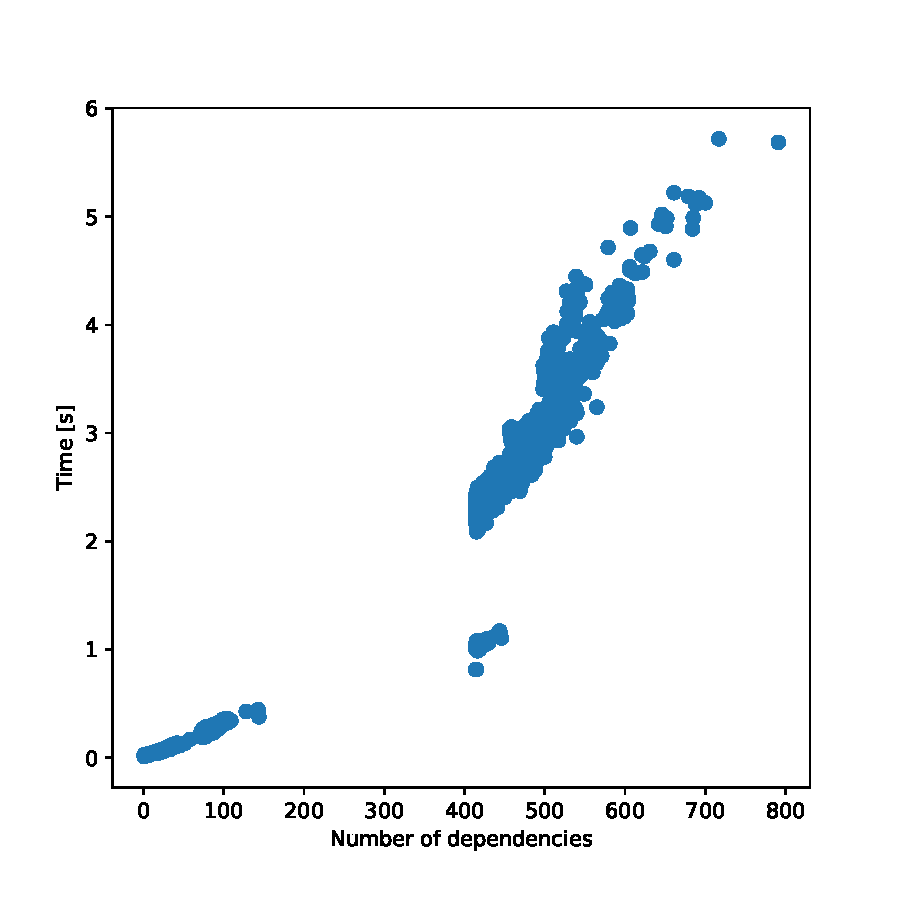
\includegraphics[width=0.32\textwidth]{figures/perf/deps_quartz_ground_fig.pdf}
    }\hfill%
    \subfloat[][Solve times]{
    \label{subfig:deps_quartz_solve}
        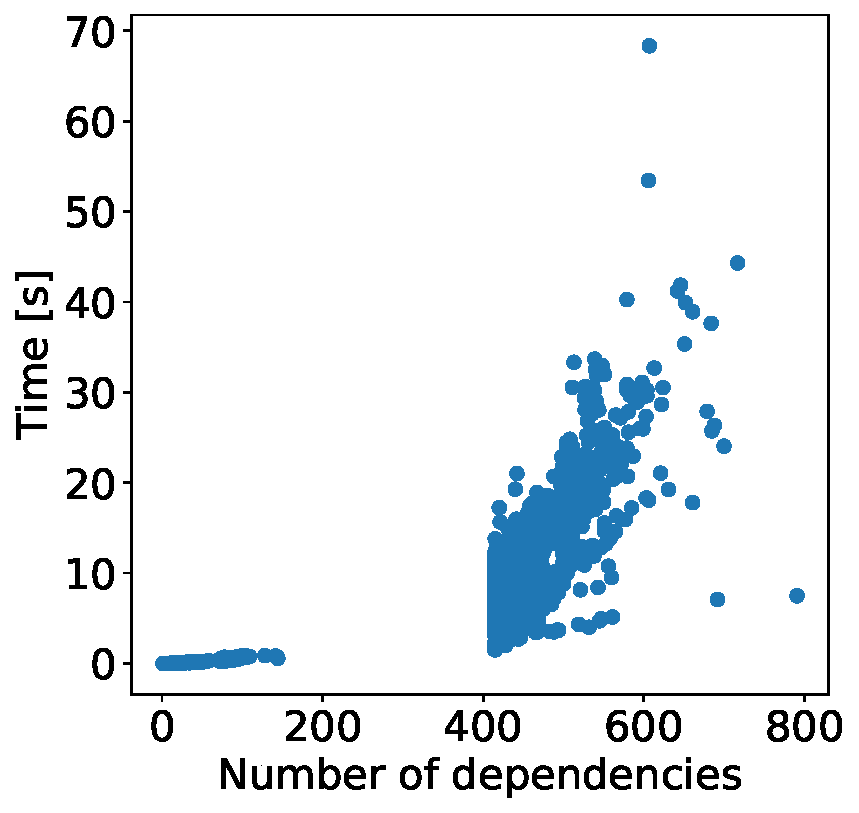
\includegraphics[width=0.32\textwidth]{figures/perf/deps_quartz_solve_fig.pdf}
    }\hfill%
    \subfloat[][Full solving times]{
    \label{subfig:deps_quartz_full}
        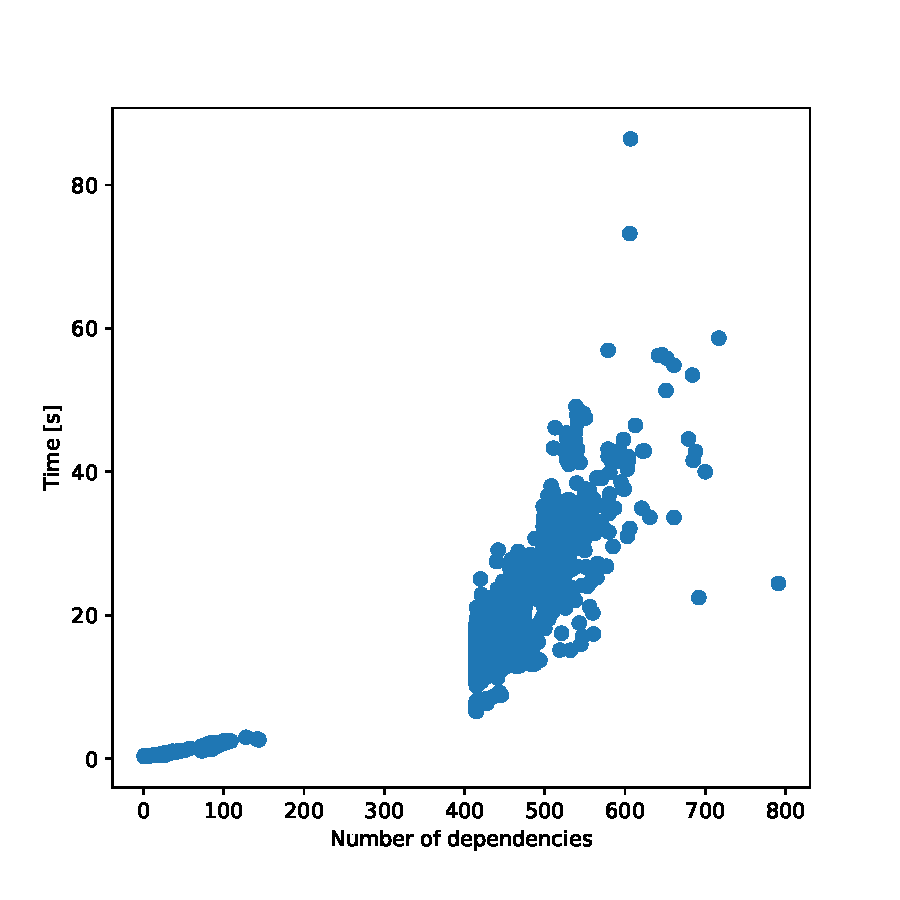
\includegraphics[width=0.32\textwidth]{figures/perf/deps_quartz_total_fig.pdf}
    }
    \caption{Solve times vs. number of dependent packages across all packages on the Quartz machine.}
    \label{fig:deps_quartz}

\end{figure*}



\begin{figure*}[htb]

    \centering
    \subfloat[][Ground times]{
    \label{subfig:deps_lassen_load}
        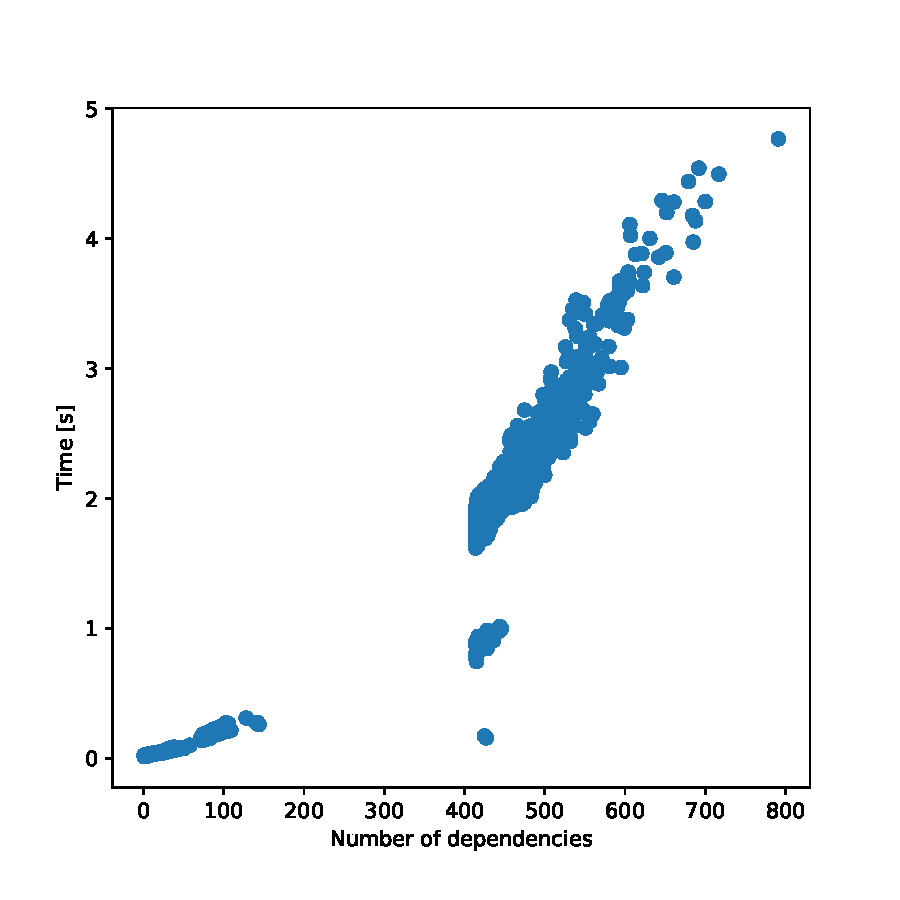
\includegraphics[width=\perfsubfigwidth\textwidth]{figures/perf/deps_lassen_ground_fig.pdf}
    }\hfill%
    \subfloat[][Solve times]{
    \label{subfig:deps_lassen_solve}
        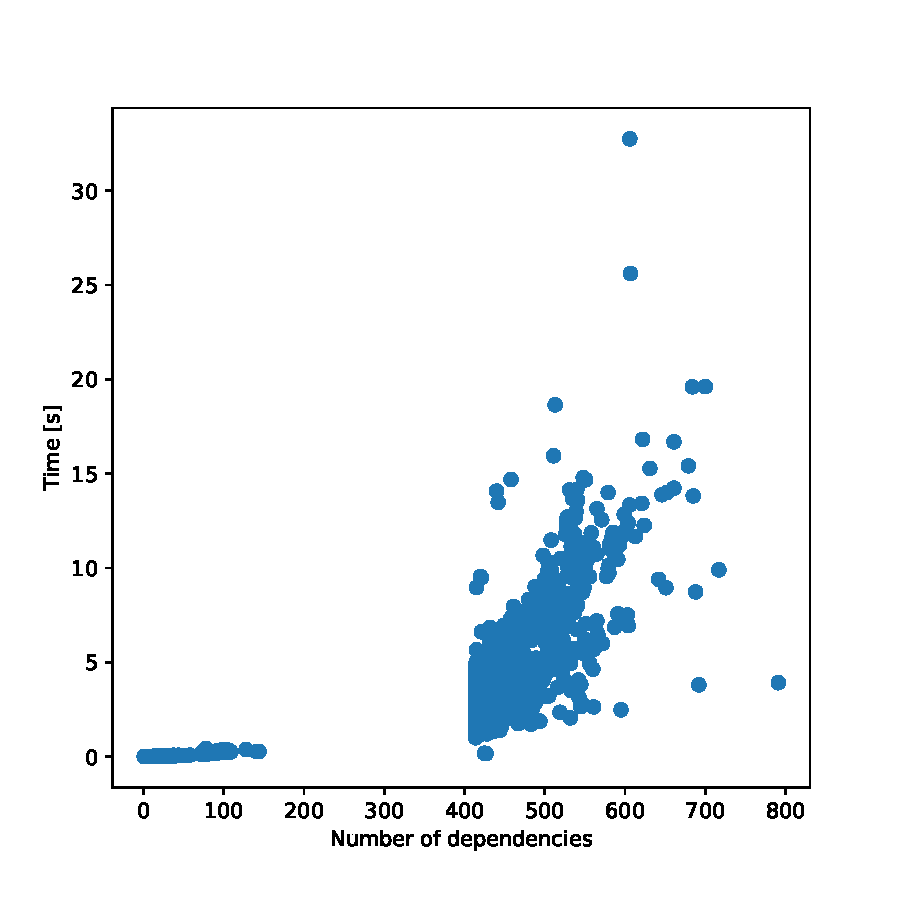
\includegraphics[width=\perfsubfigwidth\textwidth]{figures/perf/deps_lassen_solve_fig.pdf}
    }\hfill%
    \subfloat[][Full solving times]{
    \label{subfig:deps_lassen_full}
        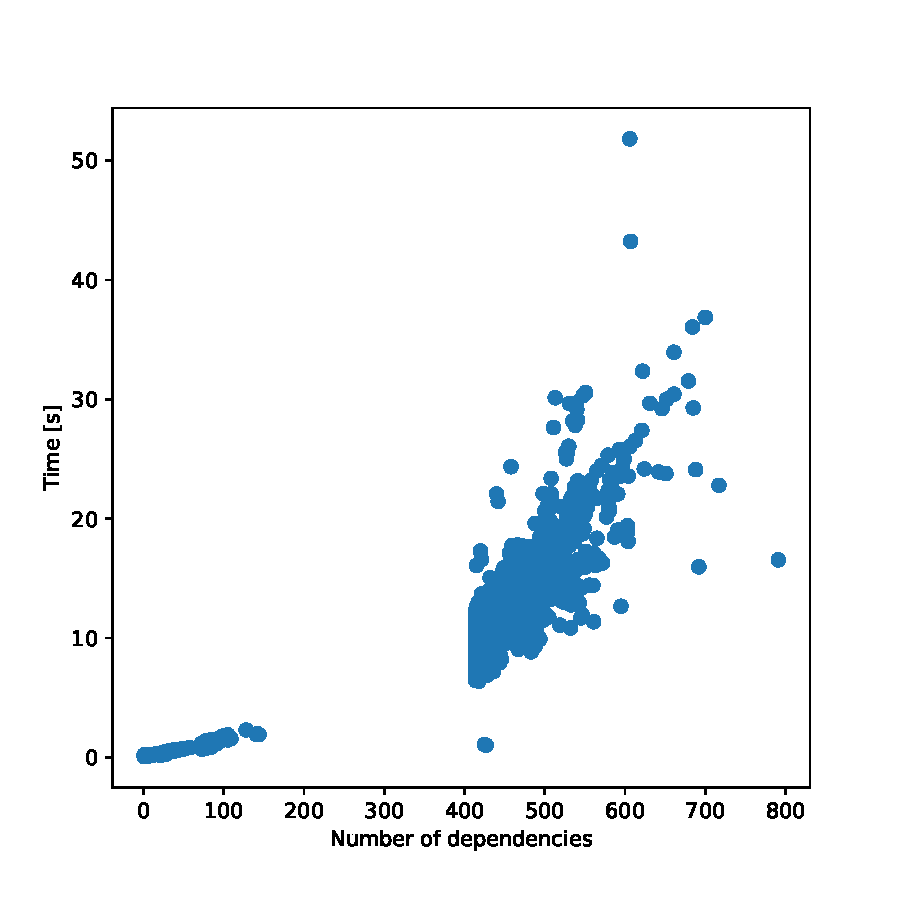
\includegraphics[width=\perfsubfigwidth\textwidth]{figures/perf/deps_lassen_total_fig.pdf}
    }
    \caption{Solve times vs. number of dependent packages across all packages on the Lassen machine.}
    \label{fig:deps_lassen}

\end{figure*}


Figures~\ref{fig:deps_quartz} and~\ref{fig:deps_lassen} show the grounding, solve, and full solving (i.e., involving all the stages) times for all the packages on Quartz and Lassen, respectively~\cite{llnl:hpc}. Quartz is an Intel-based 3.3 Petaflop cluster at Lawrence Livermore National Laboratory (LLNL). Each node comprises of two Intel Xeon E5-2695 v4 processors and 128GB of memory. The Lassen machine at LLNL is a smaller variant of Sierra, a 125 Petaflop machine. Each node on Lassen has two IBM POWER9 processors and four NVIDIA Tesla V100 (Volta) GPUs, as well as 256GB of memory. Load times, as one would expect, were not affected by the number of packages. Also, the setup times are the same order of magnitude as ground times and do not depend on \clingo{}'s performance so they were ommitted in favor of showing times that are directly dependent on \clingo{}. We used the \clingo{}'s "tweety" configuration and "usc,one" optimization strategy for running the solving process. Further below we explore the differences in solving times between these different strategies.

We can see from the figures that the time increases as the number of possible package dependencies increases. This is because increased number of possible dependencies leads to a larger number of facts and a bigger logic program overall. We measure possible dependencies rather than actual dependencies of the result because possible dependencies better measure the size of the problem space. In particular, when many packages can provide a virtual dependency like the Message Passing Interface (MPI), much of the potential solve space is not present in the final result when a single MPI implementation is chosen.

Figures~\ref{fig:deps_quartz} and~\ref{fig:deps_lassen} also show that there are two major clusters in the execution times. The clusters are separated by a gap in the possible dependencies. One cluster contains packages with less than 200 possible dependencies, whereas, the other major cluster contains packages with more than 400 possible dependencies. This natural clustering occurs because some low-level dependencies have options that can trigger huge potential dependency trees, and the gap is between packages that can include those dependencies and those that cannot.

% TODO: Can we confirm this?? My explanation above is slightly vague -- GBB
% The gap occurs because of dependency on \emph{cmake}, which itself depends cumulatively on more than 400 packages.

Besides dependencies another set of factors that influences the execution times are \clingo{} parameters. Specifically, \clingo{} defines six configuration presets: \emph{frumpy}, \emph{jumpy}, \emph{tweety}, \emph{trendy}, \emph{crafty}, and \emph{handy}. Each preset sets numerous low level parameters that control different aspects of the solver. In our performance study, we specifically focus on three configurations: \emph{tweety} -- geared towards typical ASP programs, \emph{trendy} -- geared towards industrial problems, and \emph{handy} -- geared towards large problems.


\begin{figure*}[htb]

    \centering
    \subfloat[][Ground times]{
    \label{subfig:cdf_quartz_ground}
        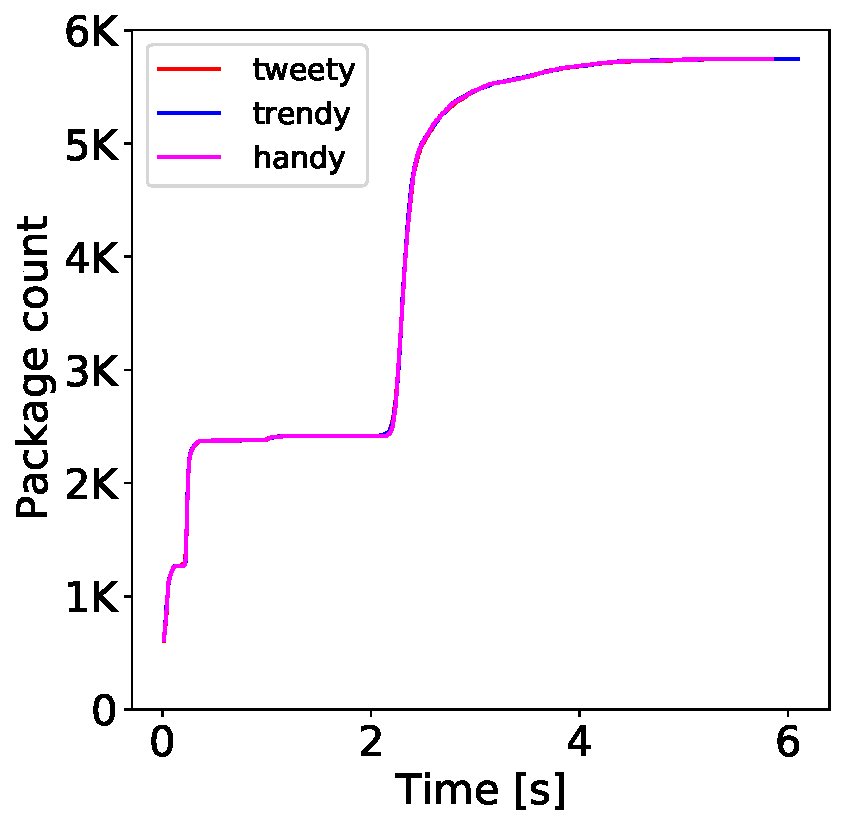
\includegraphics[width=\perfsubfigwidth\textwidth]{figures/perf/cdf_quartz_ground_fig.pdf}
    }\hfill%
    \subfloat[][Solve times]{
    \label{subfig:cdf_quartz_solve}
        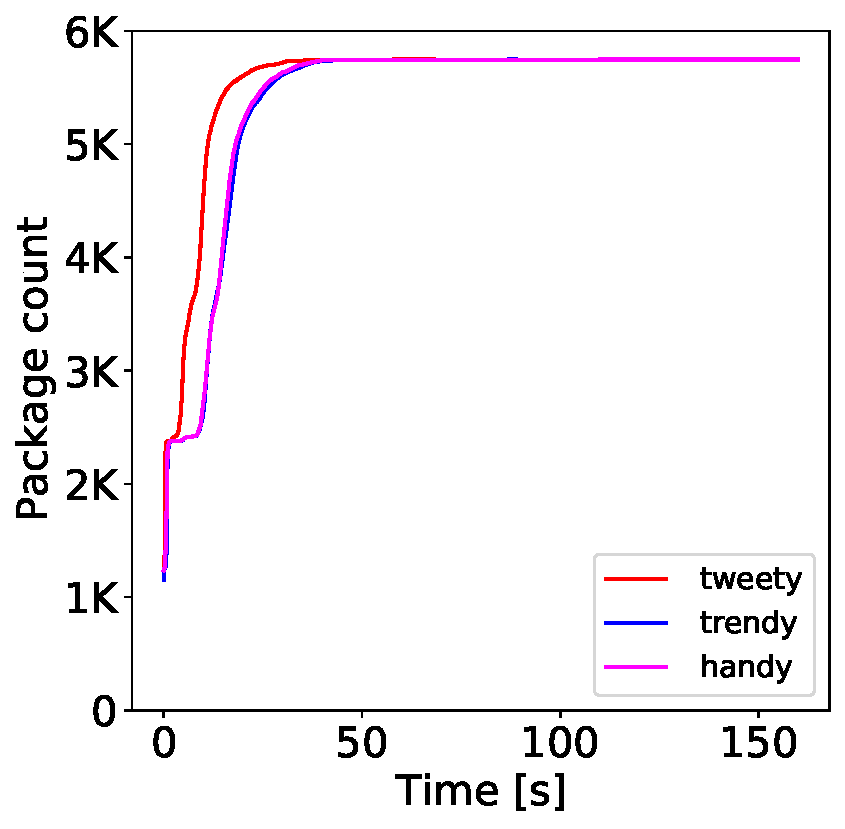
\includegraphics[width=\perfsubfigwidth\textwidth]{figures/perf/cdf_quartz_solve_fig.pdf}
    }\hfill%
    \subfloat[][Full solving times]{
    \label{subfig:cdf_quartz_full}
        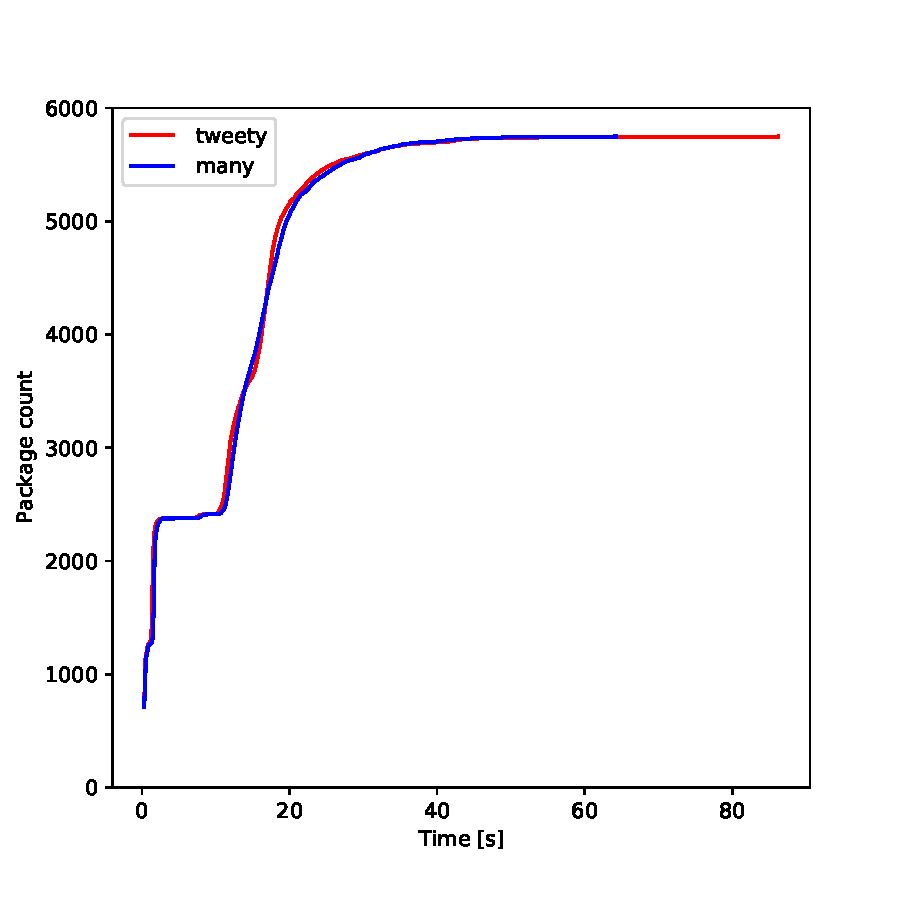
\includegraphics[width=\perfsubfigwidth\textwidth]{figures/perf/cdf_quartz_total_fig.pdf}
    }
    \caption{Cumulative distribution of solve times across all packages on the Quartz machine.}
    \label{fig:cdf_quartz}

\end{figure*}



\begin{figure*}[htb]

    \centering
    \subfloat[][Load times]{
    \label{subfig:cdf_lassen_load}
        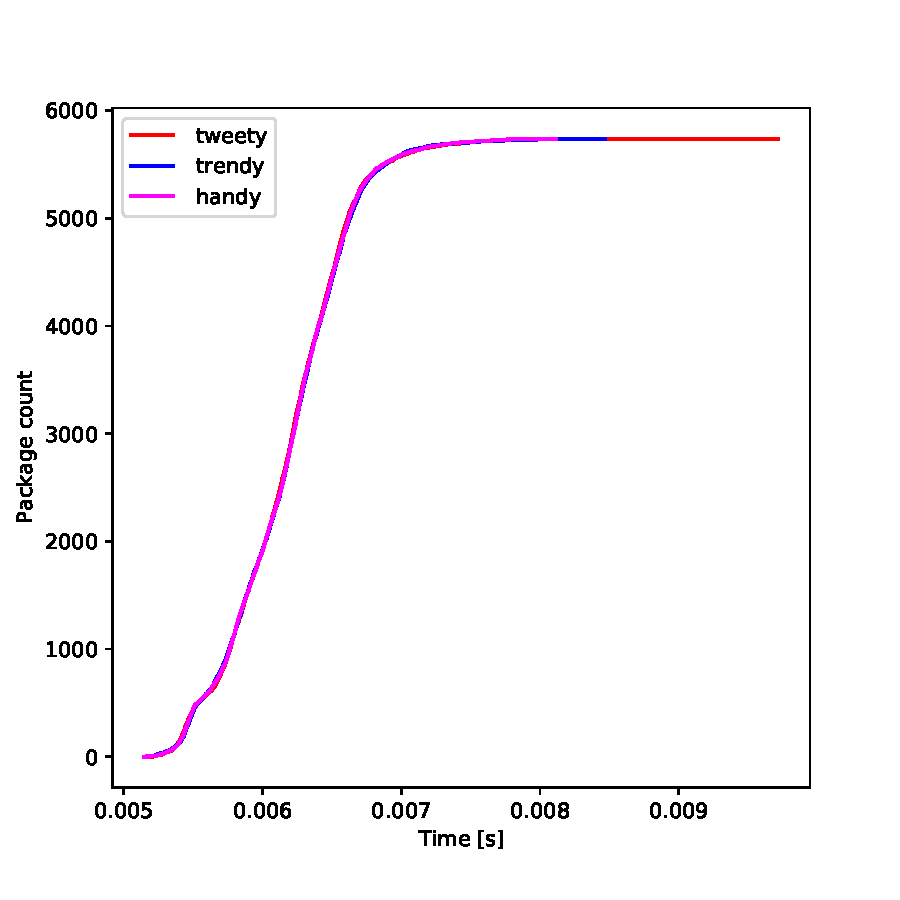
\includegraphics[width=0.32\textwidth]{figures/perf/cdf_lassen_load_fig.pdf}
    }\hfill%
    \subfloat[][Solve times]{
    \label{subfig:cdf_lassen_solve}
        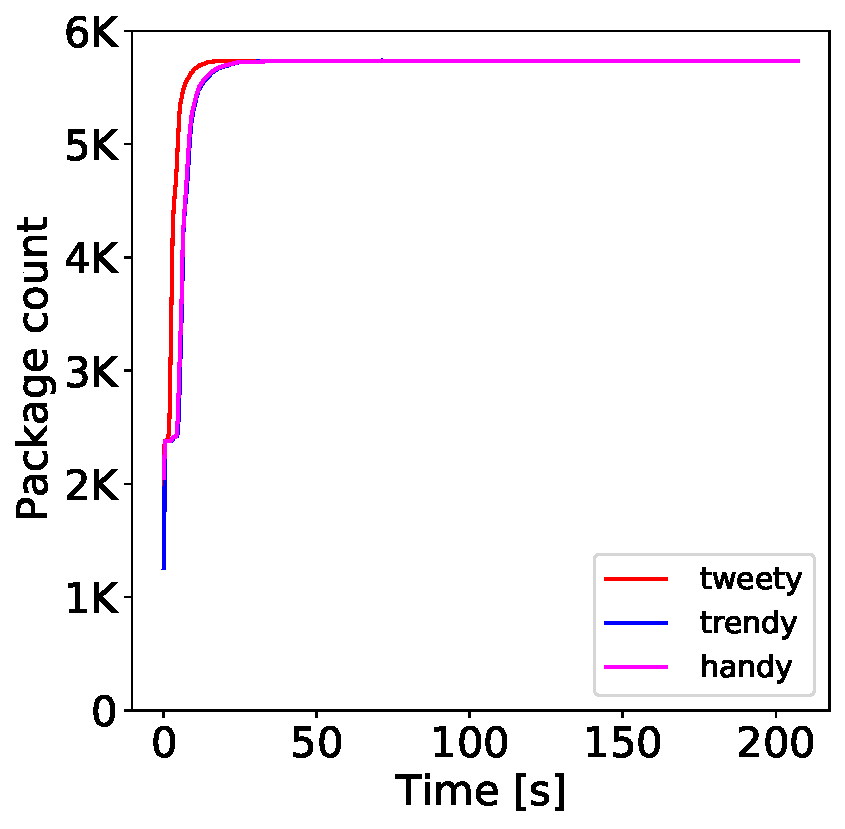
\includegraphics[width=0.32\textwidth]{figures/perf/cdf_lassen_solve_fig.pdf}
    }\hfill%
    \subfloat[][Full solving times]{
    \label{subfig:cdf_lassen_full}
        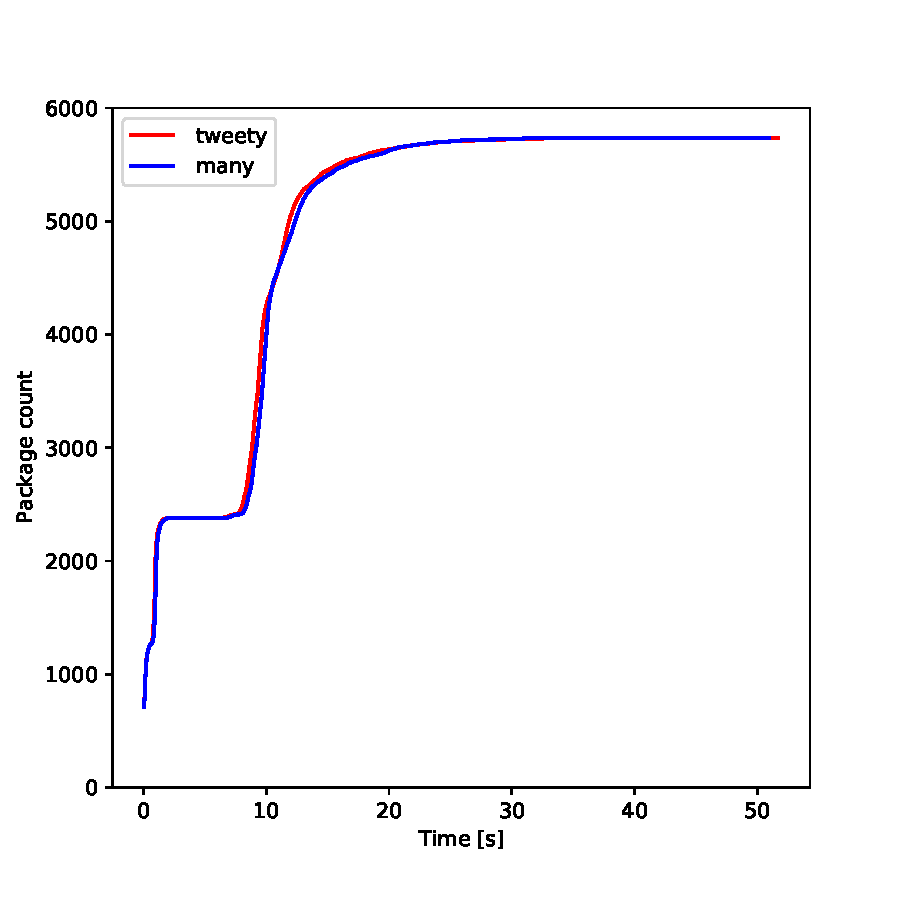
\includegraphics[width=0.32\textwidth]{figures/perf/cdf_lassen_total_fig.pdf}
    }
    \caption{Cumulative distribution of solve times across all packages on the Lassen machine.}
    \label{fig:cdf_quartz}

\end{figure*}


Figures~\ref{fig:cdf_quartz} and~\ref{fig:cdf_lassen} show the cumulative distribution of the solve times under \emph{tweety}, \emph{trendy}, and \emph{handy} configurations on Quartz and Lassen machines, respectively. The vast majority of packages are fully solved in under 25 seconds on both machines. We can also see that there is no difference in ground times between the different configurations. This suggests that most low level parameters that are tweaked by each configuration control the actual solving phase. The figures cleary indicate that \emph{tweety} performs better than the other configurations we benchmarked. This is, therefore, the default configuration used in the concretization process.

% - other properties?
% - --single-shot vs. no single-shot?
% - different tactics?

\subsection{Solve timings for all packages with reuse}

In this subsection, we examine the performance of the solver with the \emph{reuse} flag switched on. As described in Section~\ref{sec:reuse}, reusing packages in a buildcache increases the number of facts proportionally to the number of cached packages.

We specifically focus on the packages in the ECP Extreme-scale Scientific Software Stack (E4S) project~\cite{e4s}. It is a community effort to provide open source software packages for developing, deploying, and running scientific applications on HPC platforms. There are just under 600 packages in E4S, but the buildcache of the project targets different architectures, operating systems, and compilers, thereby totaling over 60K pre-compiled packages (hash signatures). We divided the buildcache into 4 groups: full buildcache (63099 packages), buildcache restricted to the \texttt{ppc64le} architecture (27160 packages), buildcache restricted to the \texttt{rhel7} OS (15255 packages), and buildcache restricted to both \texttt{ppc64le} architecture and the \texttt{rhel7} OS (6804 packages). Benchmarking across an increasing size of the buildcache provides us with a better understanding of the impact of the package resuse functionality.


\begin{figure*}[htb]

    \centering
    \subfloat[][Setup times]{
    \label{subfig:cdf_e4s_quartz_load}
        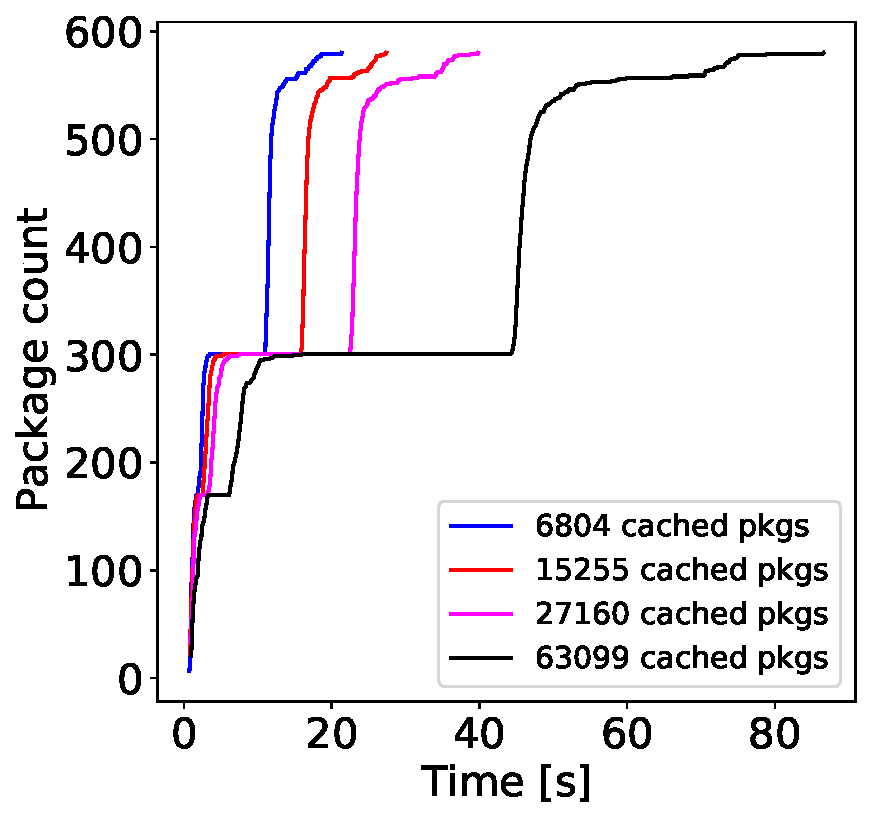
\includegraphics[width=\perfsubfigwidth\textwidth]{figures/perf/cdf_e4s_cache_quartz_setup_fig.pdf}
    }\hfill%
    \subfloat[][Solve times]{
    \label{subfig:cdf_e4s_quartz_solve}
        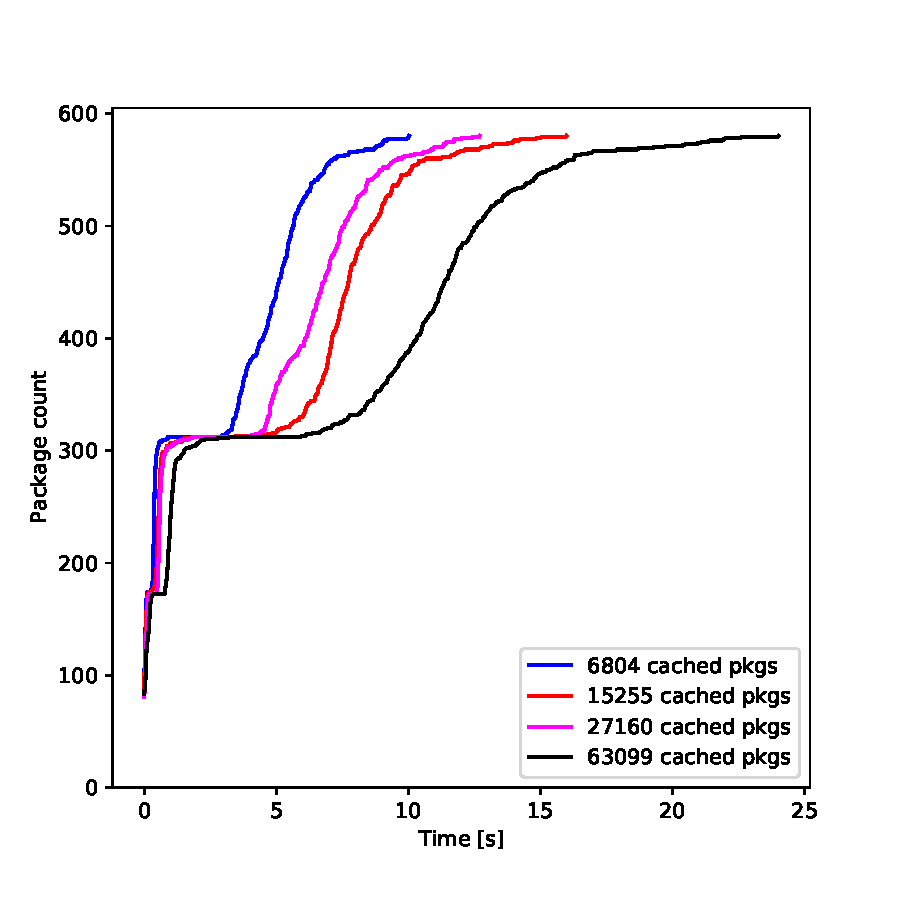
\includegraphics[width=\perfsubfigwidth\textwidth]{figures/perf/cdf_e4s_cache_quartz_solve_fig.pdf}
    }\hfill%
    \subfloat[][Total solver times]{
    \label{subfig:cdf_e4s_quartz_full}
        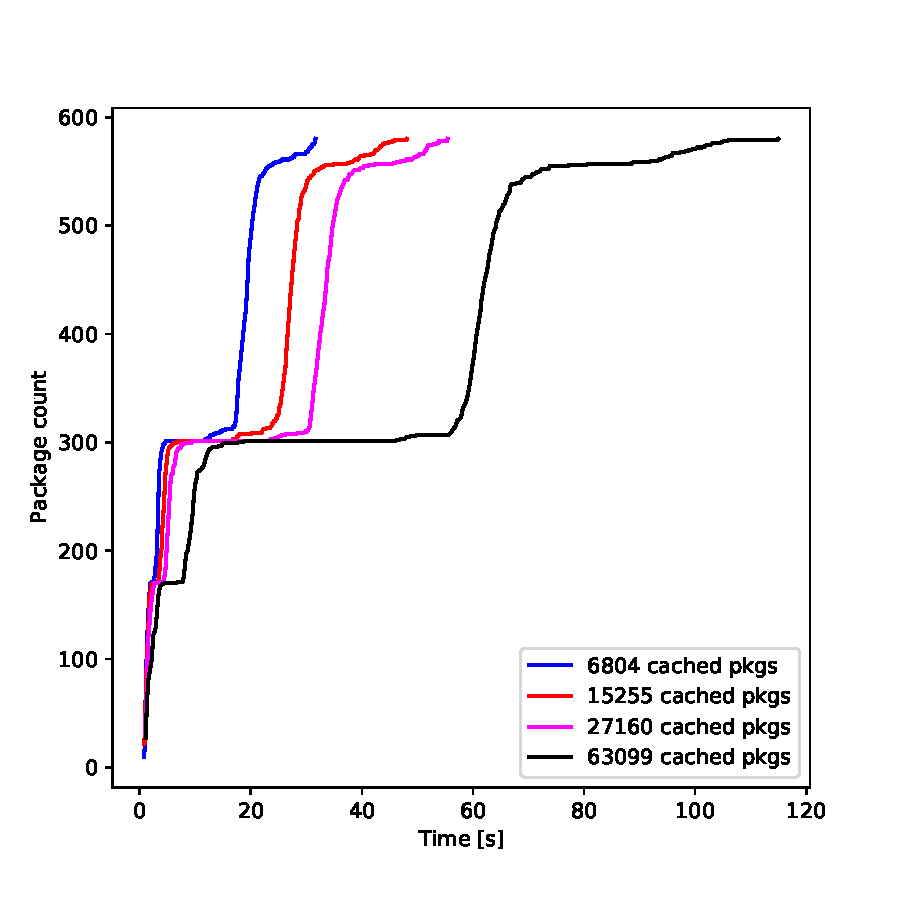
\includegraphics[width=\perfsubfigwidth\textwidth]{figures/perf/cdf_e4s_cache_quartz_total_fig.pdf}
    }
    \caption{Cumulative distribution of solve times for different cache sizes across all E4S packages on the Quartz machine.}
    \label{fig:cdf_e4s_quartz}

\end{figure*}



\begin{figure*}[htb]

    \centering
    \subfloat[][Setup times]{
    \label{subfig:cdf_e4s_lassen_load}
        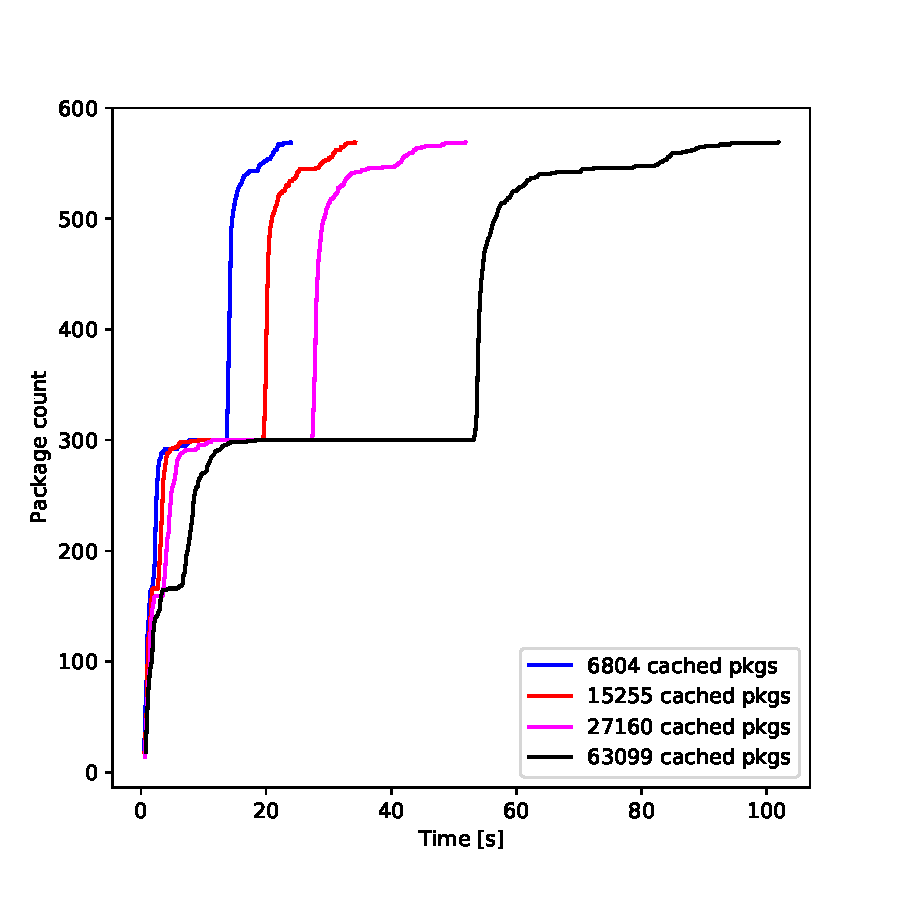
\includegraphics[width=0.32\textwidth]{figures/perf/cdf_e4s_cache_lassen_setup_fig.pdf}
    }\hfill%
    \subfloat[][Solve times]{
    \label{subfig:cdf_e4s_lassen_solve}
        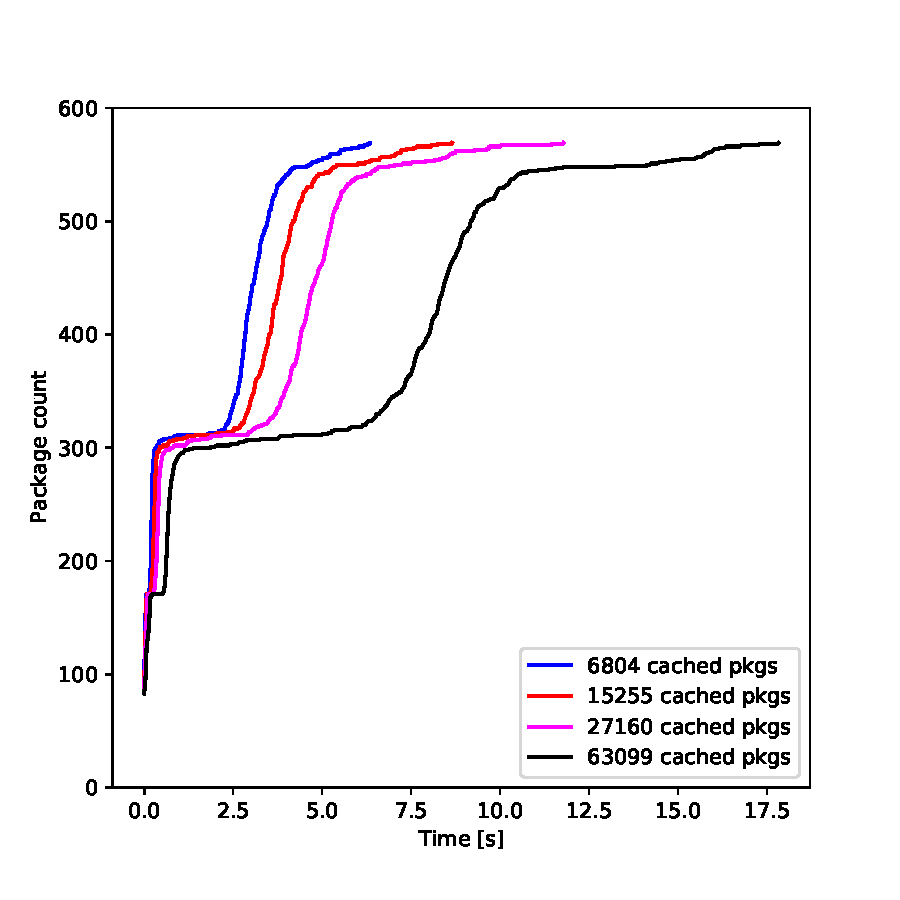
\includegraphics[width=0.32\textwidth]{figures/perf/cdf_e4s_cache_lassen_solve_fig.pdf}
    }\hfill%
    \subfloat[][Total solver times]{
    \label{subfig:cdf_e4s_lassen_full}
        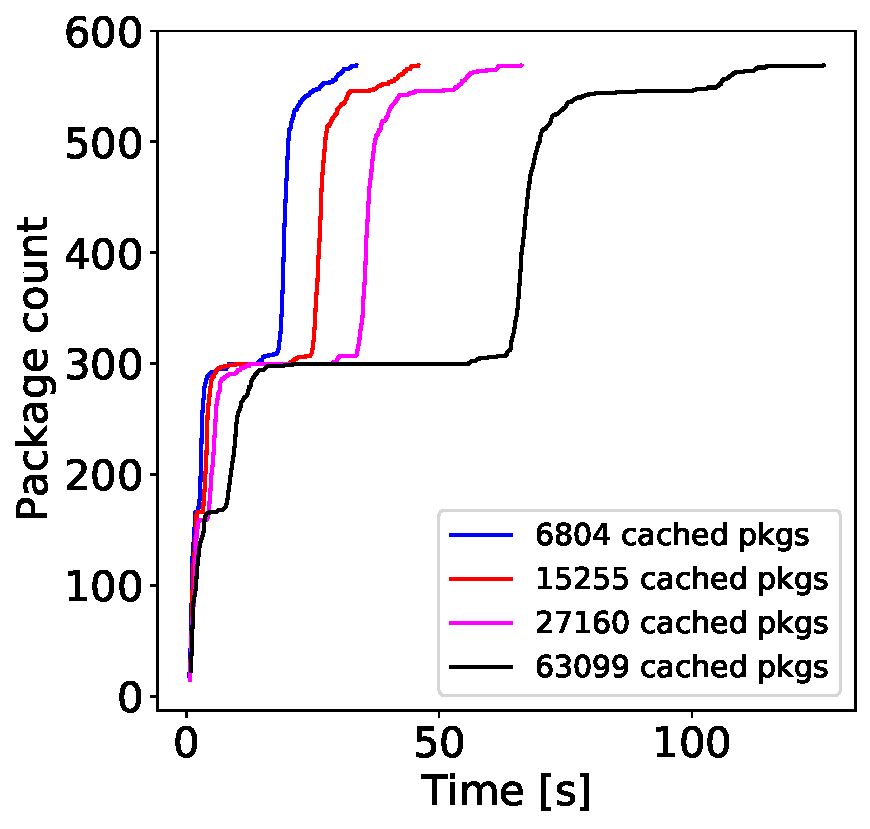
\includegraphics[width=0.32\textwidth]{figures/perf/cdf_e4s_cache_lassen_total_fig.pdf}
    }
    \caption{Cumulative distribution of solve times for different cache sizes across all E4S packages on the Lassen machine.}
    \label{fig:cdf_e4s_lassen}

\end{figure*}


Figures~\ref{fig:cdf_e4s_quartz} and~\ref{fig:cdf_e4s_lassen} show the cumulative distribution of the solve times of the E4S packages with increasing buildcache on Quartz and Lassen, respectively. We first observe that the setup times are generally higher than the actual solve times, even for smaller buildcaches. This happens because when we reuse packages we need to encode much more facts than usual, which are facts representing the dependencies. The figures also show that there is a significant jump in the solve times for the biggest buildcache. The majority of this jump occurs in the setup phase, as shown in the figures, suggesting that the runtime is being dominated by the serial process of generating facts for the solver, rather than exponential explosion in the solver. This suggests positive outcomes for future work improving performance in this area.


\section{Conclusions}
- TBD
A paragraph of text goes here. Lots of text. Plenty of interesting
text. Text text text text text text text text text text text text text
text text text text text text text text text text text text text text
text text text text text text text text text text text text text text
text text text text text text text.
More fascinating text. Features galore, plethora of promises.

%-------------------------------------------------------------------------------
\section*{Acknowledgments}
%-------------------------------------------------------------------------------
The USENIX latex style is old and very tired, which is why
there's no \textbackslash{}acks command for you to use when
acknowledging. Sorry.

%-------------------------------------------------------------------------------
\section*{Availability}
%-------------------------------------------------------------------------------

USENIX program committees give extra points to submissions that are
backed by artifacts that are publicly available. If you made your code
or data available, it's worth mentioning this fact in a dedicated
section.

%-------------------------------------------------------------------------------
% References
%-------------------------------------------------------------------------------
{
   \footnotesize
   \bibliographystyle{abbrv}
   \bibliography{\jobname}
}

%%%%%%%%%%%%%%%%%%%%%%%%%%%%%%%%%%%%%%%%%%%%%%%%%%%%%%%%%%%%%%%%%%%%%%%%%%%%%%%%
\end{document}
%%%%%%%%%%%%%%%%%%%%%%%%%%%%%%%%%%%%%%%%%%%%%%%%%%%%%%%%%%%%%%%%%%%%%%%%%%%%%%%%

%%  LocalWords:  endnotes includegraphics fread ptr nobj noindent
%%  LocalWords:  pdflatex acks
